\documentclass[10pt]{article}
\usepackage[T1]{fontenc}
\usepackage{calc}
\usepackage{setspace}
\usepackage{multicol}

\usepackage{graphicx}
\usepackage{color}
\usepackage{rotating}
\usepackage{verbatim}
\usepackage{natbib}

\setlength{\voffset}{0in}
\setlength{\topmargin}{0pt}
\setlength{\hoffset}{0pt}
\setlength{\oddsidemargin}{0pt}
\setlength{\headheight}{0pt}
\setlength{\headsep}{.4in}
\setlength{\marginparsep}{0pt}
\setlength{\marginparwidth}{0pt}
\setlength{\marginparpush}{0pt}
\setlength{\footskip}{.1in}
\setlength{\textwidth}{6.5in}
\setlength{\textheight}{8.5in}
\setlength{\parskip}{0pc}

\renewcommand{\baselinestretch}{1}

\newcommand{\bi}{\begin{itemize}}
\newcommand{\ei}{\end{itemize}}
\newcommand{\be}{\begin{enumerate}}
\newcommand{\ee}{\end{enumerate}}
\newcommand{\bd}{\begin{description}}
\newcommand{\ed}{\end{description}}
\newcommand{\prbf}[1]{\textbf{#1}}
\newcommand{\prit}[1]{\textit{#1}}
\newcommand{\beq}{\begin{equation}}
\newcommand{\eeq}{\end{equation}}
\newcommand{\beqa}{\begin{eqnarray}}
\newcommand{\eeqa}{\end{eqnarray}}
\newcommand{\bdm}{\begin{displaymath}}
\newcommand{\edm}{\end{displaymath}}
\newcommand{\script}[1]{\begin{cal}#1\end{cal}}
%\newcommand{\citee}[1]{\citename{#1} (\citeyear{#1})}
\newcommand{\citee}[1]{\citeauthor*{#1} (\citeyear{#1})}
\newcommand{\h}[1]{\hat{#1}}
\newcommand{\ds}{\displaystyle}

\newcommand{\app}
{
\appendix
}

\newcommand{\appsection}[1]
{
\let\oldthesection\thesection
\renewcommand{\thesection}{Appendix \oldthesection}
\section{#1}\let\thesection\oldthesection
\renewcommand{\theequation}{\thesection\arabic{equation}}
\setcounter{equation}{0}
}

\pagestyle{plain}


\begin{document}

\begin{titlepage}
\begin{singlespace}
\title{Learning and Judgment Shocks in U.S. Business Cycles}

\maketitle

\thispagestyle{empty}

\abstract{This paper examines the role of judgment shocks in combination with other structural shocks in explaining post-war economic volatility within the context of a New Keynesian model.  Agents form expectations using constant gain learning then augment these forecasts with judgment.  These judgments may be interpreted as a reaction to current news stories or policy announcements that would influence people's expectations.  I allow for the possibility that these judgments be informatively based on information about structural shocks, but judgment itself may also be subject to its own stochastic shocks.  I estimate a standard New Keynesian model that includes these shocks using Bayesian simulation methods.  To aid in identifying expectational shocks from other structural shocks I include data on professional forecasts along with data on output gap, inflation, and interest rates.}\newline  

\noindent \textit{Keywords}: Learning, judgment, add-factors, New Keynesian model, Metropolis-Hastings. \\
\noindent \textit{JEL classification}: C13, E31, E50.
\end{singlespace}
\end{titlepage}

\newpage

\section{Introduction}

Rational expectations with full information about quantities of relevant state variables and stochastic shocks is the most common assumption among research using models of the macroeconomy.  The assumption makes solving, evaluating, and estimating macroeconomic models possible with standard tools (albeit, still rather sophisticated), but the informational requirements and information processing requirements behind the assumption are rather extreme.  Least squares learning is a type of non-rational, adaptive expectations that attempts to use more realistic forecasting methods within the context of macroeconomic models to understand macroeconomic dynamics.  In such a framework, economic agents gather past data and use simple least squares time series techniques to form their expectations for future outcomes before making forward looking decisions (a feasible and rather simple statistical exercise). 

One drawback of least squares learning is that expectations are based only on collections of past data that are passed through some statistical procedure.  Forward looking decisions might also be well guided by relevant current events that have not yet made themselves evident in historical data.  Examples of such events include the passing of a new law, a natural disaster, a change in political landscape, a change in international trade patterns, or news of a recent technological development, just to name a few.  As soon as such events are made known through the media, optimizing economic agents would do well to immediately change their expectations and decisions accordingly.  One could argue that rational expectations captures this realistic component of expectations formation that learning does not.  Typically in dynamic stochastic general equilibrium (DSGE) models with rational expectations, the values for current stochastic shocks are known before expectations are made.  We can interpret the quantities for these stochastic shocks as precisely measured impacts the above events on the macroeconomy.

It might also happen that current events are misinterpreted, the quantified impact is misjudged, or that judgment is otherwise misinformed and not based on actual events.  One example of an exaggerated news story in recent U.S. history might be the Y2K computer bug widely discussed in the late 1990s.  The September 11, 2001, terrorist attacks may be an example of a very real event, but whose implications to economic activity may have been overestimated.  Rational expectations cannot account for such misinterpretations of news of this type.  

Judgment based on information in the news that is impractical or impossible to quantify may therefore benefit optimal decision making, be detrimental, or more probably a combination of both.  I examine within the context of a standard stochastic New Keynesian model expectations that are formed by least squares learning forecasts and are then augmented by judgment.  The least squares forecasts incorporates historical data on the output gap, inflation rate, and the federal funds rate, data that can be readily obtained and which are informative for expectations within the context of the New Keynesian model.  If expectations were rational and agents had full information, they would also use current realizations of structural shocks in forming expectations.  In the learning environment with judgment, values for structural shocks cannot be obtained or estimated, but judgments based on news and current events may incorporate some of this information.  Judgment may also be subject to its own stochastic shocks that are independent to all other shocks and state variables.  This stochastic component of judgment can be viewed as the detrimental component to using judgment; shocks that are unrelated to economic fundamentals affect agents expectations and forward looking decisions.  One of the contributions of this paper is to provide an estimate for the degree to which judgment has influenced expectations in the post-war U.S. monetary economy, and how much of this judgment is informative (that is, related to current realizations of structural shocks) and how much is disruptive (independent of structural shocks).  I further illustrate the influence judgment shocks have had on the dynamics of inflation, output, and interest rates in U.S. history, along with traditional supply, demand, and monetary policy shocks.

Before moving forward, it is prudent to define the following terms used in this paper that I give precise meanings to, perhaps using these somewhat differently than other papers in the literature:
\bd
\item \textit{Expectation}: the value agents actually expect a variable to take in the future.  This will be the sum of agents' econometric forecast and their judgment.  When taking the model to the data, \textit{expectations} are matched to median responses from the Survey of Professional Forecasters.
\item \textit{Econometric forecast}: a forecast for a future variable computed using least squares methods and past data on the output gap, inflation rate, and the federal funds rate.
\item \textit{Judgment}: sometimes referred to as ``add-factors'' in the literature.  A value that is added to agents' econometric forecasts to reflect their actual expectations of what is to come.  Judgment is a linear combination of structural shocks and judgment shocks.  
\item \textit{Structural shocks} or \textit{fundamental shocks}: traditional stochastic shocks in the New Keynesian model: a natural rate shock, a cost shock, and a monetary policy shock.  Current values of structural shocks affect macroeconomic dynamics but they have no influence on agents' econometric forecasts.  They may, however, influence judgment.
\item \textit{Judgment shocks}: stochastic shocks to judgment that are independent of the structural shocks.
\ed

\section{Related Literature}

The literature on learning specific to monetary economics can be broadly put into two categories: 1) theoretical work that examines stability of equilibria under learning versus rational expectations, and 2) empirical and descriptive research that examines the difference in macroeconomic dynamics between learning and rational expectations.  The first branch explores the conditions for expectational stability, or E-stability, on monetary policy parameters.  A model with learning that is E-stable will have expectations that converge to the rational expectations equilibrium, within the neighborhood of the rational expectations solution.  Examples papers of this type are numerous, but include \citeauthor*{bullardmitra2002} (\citeyear{bullardmitra2002}) and (\citeyear{bullardmitra2007}), \citeauthor*{eh2003} (\citeyear{eh2003b}) and (\citeyear{eh2003}), and \citee{preston2005}, just to name a few.  These papers demonstrate that conditions on monetary policy for E-stability can be different and more restrictive than conditions for determinacy (the relevant condition when expectations are rational); the implication is that the economy can become unstable and volatile if monetary policy strays from these restrictions.

Such concerns have motivated the second branch of literature which investigates whether learning can explain macroeconomic dynamics we see in the data that is not well explained by traditional rational expectations models.  \citee{ow2005} use a calibrated model with learning to demonstrate that transient inflation shocks can lead to ``inflation scares'', prolonged periods of high inflation.  Findings like these suggests that learning can explain macroeconomic persistence.  \citee{milani2007} finds evidence for this with an estimated New Keynesian model with learning.  He finds learning can explain persistence in inflation and output without the need for common ``mechanical'' sources of persistence, such as habit formation and inflation indexation which are typically augmented to rational expectations models.  Learning has also been used to explain characteristics of the ``Great Inflation'' and ``Great Moderation'', the large run-up of inflation and macroeconomic volatility in the 1970s followed by a long period of relatively moderate volatility and low inflation since 1984.  Examples of such papers include \citee{ow2005b}, \citee{primiceri2006}, \citee{bullardeusepi2005}, and \citee{bullardsingh}.

Preceding this paper, relatively little work has investigated the importance of judgment on expectations.  \citee{rsw1997} and \citee{svensson2005} demonstrate the usefulness of judgment for central bankers when making monetary policy decisions.  \citeauthor*{beh2008} (\citeyear{beh2008}) and (\citeyear{beh2010}) incorporate judgment of the kind that is purely disruptive (judgments depend exclusively on stochastic shocks that are independent of economic fundamentals) into simple monetary models and demonstrate that judgment can create ``exuberance equilibria'', a condition that is susceptible to self-fulfilling judgments even when an equilibrium is otherwise locally determinant and/or E-stable.  They go on to suggest appropriate monetary policy to prevent such unstable outcomes.   

These papers by \citeauthor*{beh2008} fall into the first branch of learning literature mentioned above: they provide theoretical evidence that expectations formed by judgment and learning can lead to economic instability.  The present work is an attempt to bring the issue to the second branch: to determine whether judgment with learning can explain characteristics of business cycle fluctuations seen in data for the post-war United States. 

\section{Model}\label{s:nk}
Learning and judgment are examined within the context of a standard New Keynesian model, a model that has been estimated at great length with rational expectations and learning to investigate the roles stochastic shocks play in explaining macroeconomic dynamics.\footnote{Notable examples using rational expectations include \citee{ireland2004} and (\citeyear{ireland_tech_2004}), \citee{nasonsmith2005}, and \citee{smetswouters2003}, (\citeyear{smetswouters2005}), and (\citeyear{smetswouters2007}), just to name a few.  Examples of estimated DSGE models with learning include \citee{milani2007}, \citee{slobodyan_wouters_2007} and (\citeyear{slobodyan_wouters_2008}).}  In this section I describe the background and log-linearization of a rational expectations version of the model.  In the next section rational expectations are replaced with expectations formed with learning and judgment.\footnote{This is perhaps the most common way to incorporate learning into dynamic macroeconomic models.  However, as \citee{marcetsargent1989} point out and \citee{preston2005} further demonstrates, this method is not consistent with learning in the microfoundations of the model because the least squares expectations operator does not follow the law of iterated expectations, a property that is assumed when solving the model.}

The model consists of three sectors that describe consumer behavior, producer behavior under imperfectly flexible prices, and monetary policy.  Optimal consumer behavior is described by with a set of equations that determine current consumption based on past consumption, interest rates, and expectations of future consumption and future inflation.  Producer behavior is modeled with a ``Phillips curve'' which predicts the inflation rate that arises from firm's optimal pricing strategies when subject to a pricing friction.  The final sector is monetary policy, which I assume to follow a standard Taylor rule where the central bank sets a nominal interest rate which responds to expectations of future output and inflation.  These equations jointly determine the dynamics of the output gap (the percentage difference between real GDP and potential GDP), the inflation rate, and the nominal interest rate.  

\subsection{Consumers}
There are a continuum of consumer types and a continuum of intermediate good producers, each on the unit interval.  Each consumer type has a specific type of labor skill that can only be hired by a corresponding intermediate good firm.  It is assumed that there many consumers of each type so that no consumer has market power over their wage.  Moreover, it is assumed that there are the same number of consumers in each type, so that the output levels of intermediate goods do not depend on the distribution of consumer types.  Different intermediate goods firms may pay different wages, so labor income may be different for each consumer type.  To simplify the model, it is further assumed that there is a perfect asset market so despite differences in labor income, all consumers choose the same level of consumption.

Each consumer of type $i\in(0,1)$ chooses consumption, $c_t$, labor supply, $n_t(i)$, and purchases of real government bonds, $b_{t}(i)$, to maximize lifetime utility,
\beq \label{eq:util} E_0 \sum_{t=0}^{\infty} \beta^t \left[ \frac{1}{1-\frac{1}{\sigma}} \xi_t \left(c_t - \eta c_{t-1}\right)^{1-\frac{1}{\sigma}} - \frac{1}{1+\frac{1}{\mu}} n_t(i)^{1+\frac{1}{\mu}} \right], \eeq
subject to the budget constraint, 
\beq \label{eq:bc} c_t + b_t(i) = \frac{1+r_{t-1}}{1+\pi_t} b_{t-1}(i) + \frac{w_t(i)}{p_t} n_t(i) + \Pi_t - \tau_t. \eeq
where $\xi_t$ is an aggregate preference shock, $w_t(i)/p_t$ is the real wage paid to type $i$ labor; $\Pi_t$ is the total value of profits consumers earn by owning stock in firms, and $\tau_t$ is the real value of lump sum taxes.  The preference parameters are the intertemporal elasticity of substitution, denoted by $\sigma \in (0,\infty)$; the elasticity of labor supply, denoted by $\mu \in (0, \infty)$; and the degree of habit formation, denoted by $\eta \in [0,1)$.  When the degree of habit formation is greater than zero, consumers' utility from current consumption depends on their previous level of consumption.  Habit formation introduces persistence in consumption, and therefore output, which is commonly found in empirical studies of DSGE models.\footnote{For example, \citee{smetswouters2005} find point estimates of habit formation close to unity.  Furthermore, \citee{fuhrer2000} finds that habit formation leads to ``hump-shaped'' impulse response functions, a characteristic commonly supported by U.S. and European data.  \citee{milani2007} finds a significant degree of habit formation, but only under rational expectations.  When estimating the model with constant gain learning, he finds an estimate for the degree of habit formation close to zero.}   

Log-linearizing consumers' first order conditions leads to the following log-linear Euler equation,
\beq \label{eq:lneuler} \h{\lambda}_{t} = E_t \h{\lambda}_{t+1} + \h{r}_t - E_t \pi_{t+1}, \eeq
where $\h{\lambda}_t$ is the percentage deviation from the steady state of the Lagrange multiplier on the budget constraint, (\ref{eq:bc}), and is therefore interpreted as the marginal utility of real income.  A hat indicates the percentage deviation of a variable from its steady state.\footnote{A hat is omitted from $\pi_t$ because it is necessary to assume the steady state level of inflation is equal to zero when deriving the log-linear supply relationship.}  Utility maximization leads to the following log-linear marginal utility of income,
\beq \label{eq:lnlambda} \h{\lambda}_t = \frac{1}{ (1-\beta \eta)(1-\eta)}\left[ \beta \eta \sigma E_t \h{c}_{t+1} - \sigma(1+\beta \eta^2) \h{c}_t + \sigma \eta \h{c}_{t-1} \right] + \left(\h{\xi}_t - \beta \eta E_t \h{\xi}_{t+1} \right). \eeq
The marginal utility of income, (\ref{eq:lnlambda}), and the Euler equation, (\ref{eq:lneuler}), make up the IS sector of the model.

\subsection{Producers}
There is one final good used for consumption which is sold in a perfectly competitive market and produced with a continuum of intermediate goods according to the production function,
\beq \label{eq:yprod} y_t = \left[ \int_0^1 y_t(i)^{\frac{\theta-1}{\theta}} di \right]^{\frac{\theta}{\theta-1}}, \eeq
where $y_t$ is the output of the final good, $y_t(i)$ is the output of intermediate good $i$, and $\theta\in(1,\infty)$ is the elasticity of substitution in production.  Profit maximization leads to the following demand for each intermediate good,
\beq \label{eq:yi} y_t(i) = \left[ \frac{p_t(i)}{p_t} \right]^{-\theta} y_t, \eeq
where $p_t(i)$ is the price of intermediate good $i$ and $p_t$ is the price of the final good.  Substituting equation (\ref{eq:yi}) into equation (\ref{eq:yprod}) leads to the following expression for the price of the final good in terms of the prices of intermediate goods,
\beq \label{eq:pfinal} p_t = \left[ \int_0^1 p_t(i)^{1-\theta} di \right]^{\frac{1}{1-\theta}}. \eeq

Each intermediate good is sold in a monopolistically competitive market and is produced according to the production function, $y_t(i) = z_t n_t(i)$, where $z_t$ is an aggregate technology shock.  It can be shown that intermediate goods firms' optimal choices for labor demand and labor market clearing leads to the following aggregate log-linear marginal cost,
\beq \label{eq:mc2} \h{\psi}_t = \frac{1}{\mu} \h{y}_t - \h{\lambda}_t - \left(\frac{1}{\mu} + 1\right) \h{z}_t. \eeq

Firm's pricing conditions are subject to the \citee{calvo1983} pricing friction, where only a constant fraction of firms are able to re-optimize their price in a given period.  The firms that are able to re-optimize their price is randomly determined, completely independently of firms' prices or any other characteristics or history.  I suppose that firms who are not able to re-optimize their price do adjust their price by a fraction, $\gamma \in [0,1)$, of the previous period's inflation rate.  A positive degree of price indexation introduces a source of persistence in inflation which is often found to be statistically significant when estimating New Keynesian models (see for example, \citeauthor*{smetswouters2005} (\citeyear{smetswouters2003}), (\citeyear{smetswouters2005}), (\citeyear{smetswouters2007}), and \citee{milani2007}).

Let $\omega \in (0,1)$ denote the fraction of firms that are not able to re-optimize their prices every period.  Since these firms are randomly determined, $\omega^T$ is the probability that a firm will not be able to re-optimize its price for $T$ consecutive periods.  A firm who is able to re-optimize chooses its price to maximize the following present discounted utility value of profits earned while the firm is unable to re-optimize its price again: 
\beq \label{eq:intprofit}
E_t \sum_{T=0}^{\infty} \left(\omega \beta \right)^{T} \frac{\lambda_{t+T}}{\lambda_t}
\left\{ \left(\frac{p_{t}(i) \pi_{t+T}^{*}}{p_{t+T}}\right) y_{t+T}(i) - \Psi\left[y_{t+T}(i)\right] \right\},
\eeq
where $\Psi\left[y_{t+T}(i)\right]$ is the real total cost function of producing $y_{t+T}(i)$ units, given the optimal decision for labor, and $\pi_{t+T}^{*} \equiv \prod_{j=1}^{T} (1+\gamma \pi_{t+j-1})$ is degree to which the firm's price is able to adjust according to inflation indexation.  It can be shown that the first order condition for $p_{t}(i)$ combined with the final good price index, equation (\ref{eq:pfinal}), leads to the log-linear Phillips equation,\footnote{It is assumed during the log-linearization that there is a steady state for the price level, which implicitly assumes the steady state level of inflation is equal to zero.}
\beq \label{eq:phillips} \pi_t = \frac{1}{1+\beta \gamma} \left[ \gamma \pi_{t-1} + \beta E_t \pi_{t+1} + \frac{\mu (1-\omega)(1-\omega \beta)}{\omega (\mu + \theta)} \h{\psi}_t \right]. \eeq

\subsection{Fully Flexible Prices}
The IS equations and Phillips equation can be re-written in terms of the difference from the outcome under fully flexible prices.  This allows the model to be taken to data on the output gap, the percentage deviation of real GDP from real potential GDP, as measured by the Congressional Budget Office.  

Let $\tilde{y}_t = \h{y}_t - \h{y}_t^f$ and $\tilde{\lambda}_t = \h{\lambda}_t - \h{\lambda}_t^f$ denote the percentage deviation of output and marginal utility from their fully flexible price outcomes, where a superscript $f$ denotes the outcome under fully flexible prices.  Under flexible prices the linearized Euler equation, (\ref{eq:lneuler}), and marginal utility of income, (\ref{eq:lnlambda}), still hold.  Using these conditions and imposing goods market clearing that consumption is equal to output implies,
\beq \label{eq:gapeuler} \tilde{\lambda}_{t} = E_t \tilde{\lambda}_{t+1} + \h{r}_t - E_t \pi_{t+1} - r_t^n, \eeq
\beq \label{eq:gaplambda} \tilde{\lambda}_t = \frac{1}{ (1-\beta \eta)(1-\eta)}\left[ \beta \eta \sigma E_t \tilde{y}_{t+1} - \sigma(1+\beta \eta^2) \tilde{y}_t + \sigma \eta \tilde{y}_{t-1} \right], \eeq
where $r_t^n$ is the percentage deviation of the natural interest rate from its steady state.  The ``natural interest rate'' is the interest rate that would occur under fully flexible prices.  I suppose that $r_t^n$ follows the stochastic exogenous process,
\beq \label{eq:natint} r_t^n = \rho_n r_{t-1}^n + \epsilon_{n,t}, \eeq
where $\epsilon_{n,t}$ is an independently and identically distributed shock.

When prices are fully flexible, it can be shown that intermediate goods firms will all choose the same price in a given period, and the marginal cost of production is constant, and therefore always will be equal to its steady state value.  Under fully flexible prices, equation (\ref{eq:mc2}) implies,
\bdm \h{\psi}_t^f = \frac{1}{\mu} \h{y}_t^f - \h{\lambda}_t^f - \left(\frac{1}{\mu} + 1\right) \h{z}_t = 0. \edm
One can solve this equation for $\h{z}_t$ and substitute it back into the equation for marginal cost, (\ref{eq:mc2}).  Plugging this expression for marginal cost into equation (\ref{eq:phillips}) yields the following Phillips curve in terms of the output gap,
\bdm \label{eq:phillips1} \pi_t = \frac{1}{1+\beta \gamma} \left[ \gamma \pi_{t-1} + \beta E_t \pi_{t+1} + \frac{(1-\omega)(1-\omega \beta)}{\omega (\mu + \theta)} (\tilde{y}_t - \mu \tilde{\lambda}_t) \right]. \edm
While this expression for the Phillips curve is not subject to a structural shock, when estimating the model it is convenient to have a shock here to avoid the problem of stochastic singularity.  The Phillips curve is amended with a cost shock so the form to be estimated is given by,
\beq \label{eq:gapphillips} \pi_t = \frac{1}{1+\beta \gamma} \left[ \gamma \pi_{t-1} + \beta E_t \pi_{t+1} + \kappa (\tilde{y}_t - \mu \tilde{\lambda}_t) + u_t\right], \eeq
where $\kappa$ is the reduced form coefficient on the marginal cost and $u_t$ is the exogenous cost shock that evolves according to,
\beq \label{eq:costpush} u_t = \rho_u u_{t-1} + \epsilon_{u,t}, \eeq
where $\epsilon_{u,t}$ is an independently and identically distributed shock.

\subsection{Monetary Policy}
The nominal interest rate is determined jointly with output and inflation by monetary policy.  In this paper I assume the monetary authority follows a \citee{taylor1993} type rule where the interest rate is set in response to expected output and expected inflation, with a preference for interest rate smoothing, according to,
\beq \label{eq:taylor} \h{r}_t = \rho_r \h{r}_{t-1} + (1-\rho_r) \left(\psi_{\pi} E_t \pi_{t+1} + \psi_y E_t \tilde{y}_{t+1} \right) + \epsilon_{r,t} \eeq
where $\rho_r \in [0,1)$ is the degree of exogenous interest rate persistence, $\psi_{\pi} \in (0,\infty)$ is the degree to which monetary policy responds to expectations of future inflation, $\psi_y \in (0,\infty)$ is the degree to which monetary policy responds to the expected output gap, and $\epsilon_{r,t}$ is an independently and identically distributed exogenous monetary policy shock with mean zero and variance given by $\sigma_r^2$.  

Alternative policy rules may replace expected inflation and output with current or lagged realizations.  For example, \citee{mccallum1997} argues that a policy rule that depends on current realizations of output and inflation does not accurately depict actual information available to central banks when monetary policy decisions are made, since it takes about a full quarter to produce actual data on real GDP and price levels.  He argues that the monetary policy rule should instead be expressed as a function of past data.  The Taylor rule in (\ref{eq:taylor}) is subject to this criticism under rational expectations, since rational expectations depend on current realizations of state variables and shocks.  It is shown in the next section, however, that expectations formed by least squares learning are functions of only past data.

\subsection{Complete Model}
The complete linear New Keynesian model is represented by the ``IS relationship'', given in equations (\ref{eq:gapeuler}) and (\ref{eq:gaplambda}); the Phillips curve in equation (\ref{eq:gapphillips}), and the Taylor rule in equation (\ref{eq:taylor}).  These equations determine the dynamics of the output gap ($\tilde{y}_t$), the marginal utility of income gap ($\tilde{\lambda}_t$), the inflation rate ($\pi_t$), and the interest rate ($\h{r}_t$).  The model so far is subject to three structural shocks: the natural rate shock, the cost push shock, and the monetary policy shock.

\section{Expectations} \label{s:exp}
\subsection{Learning}
The log-linearized model in the previous section can be expressed in the general form:
\beq \label{eq:sform} \Omega_{0} x_t = \Omega_{1} x_{t-1} + \Omega_{2} x_{t+1}^e + \Omega_{2} x_{t+2}^e + \Psi z_t, \eeq
\beq \label{eq:sformsh} z_t = A z_{t-1} + \epsilon_t \eeq
where the notation $x_{t+1}^e$ has replaced $E_t x_{t+1}$ to denote possibly non-rational expectations; $x_t$ is a vector of minimum state variables, given by  $x_t = [\tilde{y}_t~ \pi_t~ \h{r}_t]'$, and $z_t$ is a vector of structural shocks, given by $z_t = [r_t^n~ u_t~ \epsilon_{r,t}]'$.  The variable $\tilde{\lambda}_t$ can be eliminated by substituting equation (\ref{eq:gaplambda}) into equations (\ref{eq:gapeuler}) and (\ref{eq:gapphillips}), which leads to the inclusion of the two-period ahead expectation for the output gap, $E_t \tilde{y}_{t+2}$, in the IS equation.  The minimum state variable (MSV) solution under rational expectations is given by,
\beq \label{eq:msvsol} E_t x_{t+1} = G x_{t} + H E_t z_{t+1}, \eeq
where the elements of the matrices $G$ and $H$ are a function of the parameters of the model and may be determined by the method of undetermined coefficients.  Agents that learn do not know the the parameters that govern the economy, but do use this reduced form as their forecasting model.  Agents' information sets are restricted only to past data on $x_t$, so they are unable to collect data on past structural shocks to estimate matrix $H$.  

In period $t$ agents are able to assemble data sets only through period $t-1$.  At this point the agents estimate $G$ using least squares and use the model to make econometric forecasts for future output and inflation.  There is no constant term in the general form of the model, equation (\ref{eq:sform}), or in the rational expectation, given in equation (\ref{eq:msvsol}), since all variables are expressed in terms of percentage deviations from the steady state or flexible price outcome.  Since agents are not endowed with information about the parameters of the model to determine steady state values, it is realistic to suppose that agents also estimate a constant term in equation (\ref{eq:msvsol}).  Let $\h{G}_t^*$ denote agents' time $t$ estimate for the columns of matrix $G$ and a column for a constant term so that $\h{G}_t^* = [\h{g}_{t}~ \h{G}_t]$, where $\h{g}_{t}$ is the time $t$ estimate of the constant term. 

If agents use ordinary least squares (OLS), then,
\beq \label{eq:Gsum} \left(\hat{G}_t^*\right)' = \left( \frac{1}{t-1} \sum_{\tau=1}^{t-1} x_{\tau-1}^* {x_{\tau-1}^{*}}' \right)^{-1} \left( \frac{1}{t-1} \sum_{\tau=1}^{t-1} x_{\tau-1}^* x_{\tau}' \right), \eeq 
where $x_t^{*'} = [1~ x_t']$ is the vector of explanatory variables including the constant.  This equation can be conveniently rewritten in the following recursive form:
\beq \label{eq:lnG} \hat{G}_t^* = \hat{G}_{t-1}^* + g_t (x_{t-1} - \hat{G}_{t-1}^* x_{t-2}^*) {x_{t-2}^*}' R_t^{-1} ,\eeq
\beq \label{eq:lnR} R_t = R_{t-1} + g_t (x_{t-2}^* {x_{t-2}^*}' - R_{t-1}), \eeq
where $g_t=1/(t-1)$ is the learning gain.\footnote{To show this, let $R_t = \frac{1}{t-1} \sum_{\tau=1}^{t-1} x_{\tau-1}^* x_{\tau-1}^{*'}$ and $\left(\hat{G}_t^*\right)' = R_t^{-1} \left( \frac{1}{t-1} \sum_{\tau=1}^{t-1} x_{\tau-2}^* x_{\tau-1}' \right)$.}
The recursive form shows precisely how expectations are adaptive.  The term enclosed in parentheses in equation (\ref{eq:lnG}) is the realized forecast error using the previous estimate $\hat{G}_{t-1}^*$.  The degree to which agents adjust their expectations depends on the size of this forecast error, the variance of the estimated coefficients, captured by the inverse of matrix $R_t$, and the size of the learning gain, $g_t$.  The larger is the learning gain, the more expectations respond to the latest forecast error.  When agents use OLS, $g_t$ approaches zero as time approaches infinity.  Under constant gain learning, $g_t$ remains at some constant level, $g$, so the degree to which new observations can affect expectations is always the same.  

Agents use the least squares estimate of the coefficients in $G$ to form the econometric forecasts,
\beq \label{eq:agfore} \begin{array}{c} 
\ds E_t^* x_{t+1} = \h{g}_{t} + \h{G}_t E_t^* x_t = (I + \h{G}_t)\h{g}_{t} + \h{G}_t^2 x_{t-1}, \\ [1pc]
\ds E_t^* x_{t+2}  =\h{g}_{t} + \h{G}_t E_t^* x_{t+1} = \left[ I + \h{G}_t (I + \h{G}_t) \right] \h{g}_{t} + \h{G}_t^3 x_{t-1},
\end{array} \eeq
where $E_t^*$ denotes expectation that is equal to the econometric forecast.

\subsection{Judgment}
Agents are not able to collect realizations of stochastic shocks, $z_t$, in their forecasts.\footnote{Central banks do use a number of such sophisticated models that incorporate the presence of latent structural shocks when forming forecasts.  \citee{rsw1997} and \citee{svensson2005} point out that judgment is nonetheless an important component of central bank expectations and decisions.}  However, current events may reveal some noisy information about structural shocks, which becomes part of judgment when forming expectations.  Examples of such events may be the announcement of technological innovations, natural disasters, onset of war or political instability among trading partners, changes in weather effecting agricultural production, etc.  The news of such events cannot be instantly mapped to data to make econometric forecasts, but it is nonetheless valuable information when forming expectations.  Let agents' final expectations be the following sum of the econometric forecast given in equation (\ref{eq:agfore}) and judgment,
\beq x_{t+1}^e = E_t^* x_{t+1} + \eta_{t}, \eeq
where $\eta_t$ is an appropriately sized vector whose non-zero elements are values for judgment concerning the future output gap ($\eta_{y,t}$) and future inflation rate ($\eta_{\pi,t}$).  The judgment vector depends on current events that includes some information about $z_t$, but it also includes expectational shocks, its own stochastic component that is independent of economic fundamentals.  Let judgment evolve according to,
\beq \label{eq:news} \begin{array}{c} \ds \eta_t = \Phi z_t + \zeta_t, \\ [1pc]
 \ds \zeta_{y,t} = \rho_{\zeta,y} \zeta_{y,t-1} + \xi_{y,t}, \\ [1pc]
 \ds \zeta_{\pi,t} = \rho_{\zeta,\pi} \zeta_{\pi,t-1} + \xi_{\pi,t},
\end{array} \eeq
where matrix $\Phi$ captures the degree to which judgment successfully picks up information about structural shocks and $\zeta_t$ is a vector of autocorrelated disturbances to the judgment variables.  The second and third equations allow these disturbances to be autocorrelated so that agents' ill-informed judgment about a particular variable may persist for multiple quarters depending on the parameters $\rho_{\zeta,y}$ and $\rho_{\zeta,y}$.  The judgment shocks $\xi_{y,t}$ and $\xi_{\pi,t}$ are independently and normally distributed with mean zero and standard deviation given by $\sigma_{\xi,y}$ and $\sigma_{\xi,\pi}$, respectively.  

The structural form for evolution of judgment in equation (\ref{eq:news}) is quite general and allows as special cases common specifications for expectations in DSGE models.  If $\rho_{\\zeta,y} = \rho_{\zeta,y} = 0$ and $Var(\xi_{y,t}) = Var(\xi_{\pi,t}) = 0$ then expectations are not subject to judgment shocks.  If $\Phi=0$, then stochastic shocks are always unobservable when forming expectations, which is a common assumption among empirical learning papers.  If $\Phi=HA$, where $H$ is the coefficient on expected shocks in the MSV solution in equation (\ref{eq:msvsol}) and $A$ is the degree of persistence of structural shocks given in (\ref{eq:sformsh}), then agents are capable of observing quantities for structural shocks and the influence these shocks have on expectations is equal to the rational expectations solution.  In fact, the entire model encompasses rational expectations as a special case when these conditions are met, the learning gain is equal to zero ($g=0$), and the initial condition for learning coefficients, $G_t^*$ in equation (\ref{eq:lnG}), is consistent with the MSV solution, $G$ in equation (\ref{eq:msvsol}).  This initial condition is estimated using pre-sample data as described in the next section, and all other parameters mentioned here are estimated jointly with the New Keynesian structural parameters, so this framework can be viewed as quite unrestricted.

\section{Estimation}

The model is estimated using U.S. quarterly data from 1968:Q3 through 2007:Q1 on the output gap (percentage difference between real GDP reported by the Bureau of Economic Analysis and the measure of potential real GDP from the Congressional Budget Office), the inflation rate of the GDP deflator, and the Federal Funds Rate.  Quarterly data from the same period on one quarter ahead expectations from the Survey of Professional Forecasters is also used to help identify the parameters of the learning and judgment process.  The median responses were obtained for the one quarter ahead forecast for real GDP and the GDP deflator.  The expectation for the output gap is found by computing the percentage difference between the forecast for real GDP and the CBO estimate for potential GDP in the next quarter.  The expectation for inflation is found by computing the percentage difference between the forecast for the GDP deflator next period and the current GDP deflator.  The base year used for the forecasts from the Survey of Professional Forecasters changes throughout the sample, so the data was first appropriately rescaled.

\subsection{State Space Representation}

Equations (\ref{eq:sform}), (\ref{eq:sformsh}), (\ref{eq:lnG}), (\ref{eq:lnR}), (\ref{eq:agfore}), and (\ref{eq:news}) can be combined into following single state equation convenient for evaluating a Kalman filter,\footnote{Habit formation causes the two period ahead expectation, $\tilde{y}_{t+2}^e~$ to appear in the model, which in turn requires an evaluating a time $t$ expectation for judgment $\eta_{y,t+1}$.  For simplicity, I suppose this judgment is formed using the mathematical expectation operator on the equations in (\ref{eq:news}), advanced to period $t+1$.  This implies that when using judgment for expectations two periods ahead, agents already discount this judgment depending on the degree of persistence, $\rho_{\zeta,y}$; and the degree to which stochastic shocks $z_t$ impact judgment two periods ahead is determined by the actual degree of persistence dictated persistence of the natural rate and cost-push shocks (given by parameters $\rho_n$ and $\rho_u$).}
\beq \label{eq:state} s_t = f_t + F_t s_{t-1} + v_t \eeq
where $s_t = [\tilde{y}_t~ \pi_t~ \h{r}_t~ \tilde{y}_{t+1}^e~ \tilde{y}_{t+2}^e~ \pi_{t+1}^e~ \eta_{y,t}~ \eta_{\pi,t}~ r_t^n~ u_t~ \zeta_{y,t}~ \zeta_{\pi,t}]'$ is a vector of state variables, and $v_t = [\epsilon_{n,t}~ \epsilon_{u,t}~ \epsilon_{r,t}~ \xi_{y,t}~ \xi_{\pi,t}]$ is a vector of all the independently and identically distributed stochastic shocks.  The time-varying component of vector $f_t$ and matrix $F_t$ comes from the coefficients in $\h{g}_t$ and $\h{G}_t$ determined by the learning process in (\ref{eq:agfore}).  Since $f_t$ and $F_t$ depend only on lagged realizations of some of the state variables, they can be treated as predetermined when evaluating the Kalman filter.

Let $GAP_t$ denote the data on the output gap, $INF_t$ denote data on inflation, $FF_t$ denote data on the Federal Funds Rate, and $SPF\_GAP_t$ and $SPF\_INF_t$ denote data on expected one-quarter ahead output gap and inflation rate, respectively, implied by the Survey of Professional Forecasters.  The observation equations are given by,
\beq \begin{array}{l} \label{eq:obs}  
\ds GAP_t = 100 \tilde{y}_t, \\
\ds INF_t = \pi^{*} + 400\pi_t, \\
\ds FF_t = r^{*} + \pi^* + 400\h{r}_t.\\
\ds SPF\_GAP_t = 100 \tilde{y}_{t+1}^e, \\
\ds SPF\_INF_t = \pi^{*} + 400\pi_{t+1}^e. \\
\end{array}
\eeq
The state variables are multiplied by $100$ to convert decimals to percentages, and the inflation rate, expected inflation rate, and federal funds rate are multiplied by $4$ to convert quarterly rates to annualized rates.  The New Keynesian model assumes that the steady state inflation rate is equal to zero, but since this is not likely the case in the data, the annualized steady state inflation rate, given by  $\pi^*$, is included in the observation equations above.  The steady state gross real interest rate is set equal to the inverse of the discount factor; therefore $r^* = 400(1-1/\beta)$.  These steady state parameters are calibrated to $\pi^*=3.4$ and $\beta=0.9956$ so the steady state values match the average inflation rate and nominal interest rate in the sample.

\subsection{Initial Conditions}

Aside from standard initial conditions for the Kalman filter, it is necessary to specify initial conditions for $\h{G}_{0}^{*}$ and $R_{0}$, the initial values for learning process given in equations (\ref{eq:lnG}) and (\ref{eq:lnR}).  I use pre-sample data from 1954:Q2 through 1968:Q2 on the output gap, inflation rate, and federal funds rate and and transform these into the same terms as the state vector, $x_t$, according to,
\bdm \begin{array}{l}
\ds \tilde{y}_t = \frac{1}{100} GAP_t, \\ [1pc]
\ds \pi_t = \frac{1}{400} (INF_t - \pi^{*}), \\ [1pc]
\ds \h{r}_t = \frac{1}{400} (FF_t - r^{*} - \pi^*).
\end{array}
\edm
I estimate a VAR(1) (the same reduced form as used in the least squared learning process described in Section {\ref{s:exp}) on this data using ordinary least squares to set initial values for the learning matrices.  The coefficients from the regression are used to initialize $\h{G}_{0}^{*}$, and the elements from the sum of squares component of the estimate of the variance of the coefficients is used to initialize $R_{0}$.

\subsection{Bayesian Estimation}

Table \ref{tb:parms} lists the parameters to be estimated, along with the prior distribution imposed for Bayesian estimation.  The parameters include the learning gain, the parameters of the New Keynesian Model described in Section \ref{s:nk}, the coefficients $\Phi$ in equation (\ref{eq:news}) governing how stochastic shocks informatively impact judgment, the persistence of stochastic components to judgment, also in equation (\ref{eq:news}), and the standard deviation of the structural shocks and judgment shocks. 

The model is estimated with Bayesian methods using the Metropolis-Hastings algorithm.  The vector of parameters were drawn from the posterior distribution 400,000 times and the first 100,000 draws were discarded for a burn-in period.  Table \ref{tb:parms} shows the prior distributions used for the estimation.  The prior distributions for the New Keynesian parameters are similar to others used in the literature.  The prior mean for the learning gain is set to 0.02, with a rather large standard deviation of 0.03 which allows for a wide range for learning dynamics.  The value of the learning gain two standard deviations above the mean is 0.08, which means agents econometric estimates evolve very quickly and the approximate sample size agents to develop their econometric estimates is only $0.08^{-1} = 12.5$ (just over 3 years of data).  The large standard deviation for the prior on the learning gain also allows for a relatively large probability that the learning gain is close to zero, implying agents use a very large number of observations and agents adjust their econometric estimates only very slowly.  Finally, the prior distributions for the coefficients in judgment process are intentionally made very wide in recognition that no previous literature has attempted to measure or even discuss such coefficients.  The priors for these coefficients are normal with zero mean and standard deviation equal to 4.0.   

\section{Results}
\subsection{Parameters}
The prior and posterior distributions for the parameters are listed in Table \ref{tb:parmsest}.  The last three columns present the median, 5th percentile and 95th percentile of the posterior distributions for the parameters.  The estimate for the learning gain is found to be 0.0322 with a relatively tight posterior distribution relative to the prior.  This implies that agents use approximately $0.0322^{-1} = 31.06$ observations for forming least squares forecasts, which corresponds to about 7.75 years.  This is a magnitude similar to that found by \citee{milani2007}, and \citee{slobodyan_wouters_2007} and (\citeyear{slobodyan_wouters_2008}).  Habit formation is found to be a significant source of persistence, with an estimate $\eta=0.6871$.  Price indexation is found to be less important in explaining persistence with an estimate $\gamma=0.2462$.  Other significant sources of persistence come from the natural rate shock ($\rho_n = 0.95$), cost shock ($\rho_u=0.78$), and the persistence of disturbances to judgment on output and inflation, with $\rho_{\zeta,y}=0.94$ and $\rho_{\zeta,\pi}=0.89$, respectively.  Only the preference parameters $\sigma$ and $\mu$ are poorly identified by the data; these posterior distributions largely mirror the priors. 

\subsection{Judgment}
The posterior distributions for the coefficients in $\Phi$ for the judgment process are very significantly informed by the data; these posterior distributions are considerably tight given the very wide prior distributions.  Recall the parameters in $\Phi$ determine how much judgment depends on actual stochastic shocks.  Using equation (\ref{eq:news}), the variance of judgment can be decomposed into variance caused by structural parameters (informed judgment) and variance from the independent stochastic component (judgment shocks) as follows,
\beq \label{eq:newsdecomp} Var(\eta_t) = \Phi Var(z_t) \Phi' + Var(\zeta_t). \eeq
Both $z_t$ and $\zeta_t$ are autoregressive stochastic processes whose variances depend on the variances for the shocks.  To illustrate, the variance for $z_t$ can be derived from the variance of the underlying independently and identically distributed shocks using equation (\ref{eq:sformsh}) as follows,
\bdm Var(z_t) = A Var(z_{t-1}) A' + Var(\epsilon_t) \edm
Since the variance of $z_t$ does not depend on time, we can solve for this variance using the $vec()$ operator on both sides of this equation,
\bdm vec(Var(z_t)) = A \otimes A vec(Var(z_t)) + vec(Var(\epsilon_t)). \edm
Solving leads to the expression,
\beq \label{eq:newsdcomp} vec(Var(z_t)) = (I - A \otimes A)^{-1} vec(Var(\epsilon_t)). \eeq
The off-diagonal elements of $Var(\epsilon_t)$ are zero, and the diagonal elements are given by squares of $\sigma_n$, $\sigma_u$, and $\sigma_r$, whose estimates are reported in Table \ref{tb:parmsest}.  The output $vec(Var(z_t))$ is then appropriately re-sized to yield $Var(z_t)$ to substitute into equation (\ref{eq:newsdecomp}).  A symmetric exercise performed on the autoregressive equations in (\ref{eq:news}) yields $Var(\zeta_t)$.  

Given the estimates for these variances, equation (\ref{eq:newsdcomp}) can be used to determine what percentage of the variability in output and inflation depends on structural shocks and judgment shocks.  Table \ref{tb:newsdec} reports these results.  About 85\% of the variability judgment in output is explained by the variance of the shock to judgment and the remaining 15\% of variability is explained primarily by the variance of the natural rate shock.  This implies judgment on output is primarily ill-informed: only a small amount of judgment is based on information related to fundamentals in the economy.  The second column of Table \ref{tb:newsdec} shows the result is very similar for judgment regarding inflation.  About 62\% of the judgment in inflation is ill-informed, and the remaining 38\% depends on information from the cost shock.  The impact of monetary policy shocks on judgment of both variables was essentially equal to zero.

Its interesting that both the natural rate shock and cost shock help inform judgment, but strangely, the natural rate shock is not used for judgments regarding inflation, and the cost shock is not used for judgments regarding output.  Both of these shocks influence output and inflation in equilibrium - yet agents mistakenly believe that cost shocks only drive inflation, and natural rate shocks only drive output.

\subsection{Impulse Responses}
Impulse response functions cannot be computed in quite the same way in models with learning as models with rational expectations.  Learning adds a non-linearity to the model: the coefficients on the state equation, (\ref{eq:state}), have a time $t$ subscript which depend on the state of the state of the learning process, represented by matrices $\hat{G}_t^*$ and $R_t$ in equations (\ref{eq:lnG}) and (\ref{eq:lnR}), respectively.  The responses to structural shocks depend on the state of the learning process and are therefore time-dependent.  Moreover, unlike a rational expectations model, a model with learning evolves absent of any shocks when learning matrices $\hat{G}_t^*$ and $R_t$ are away from the rational expectations solution.  Expectations continue to evolve with new incoming data, causing movements in output, inflation, and interest rates even when all shocks are set equal to zero.\footnote{When the model is E-stable and in the neighborhood of the rational expectations solution, then absent of shocks $\hat{G}_t^*$ and $R_t$ trend towards the rational expectations solution over time.}  To identify the impact a shock has in this ever-changing environment, I simulate the model using the state equation (\ref{eq:state}) with all shocks for all time periods set to zero.  I then simulate the model with a one standard deviation impulse shock.  In the first period only one shock is set equal to its standard deviation and all other shocks are set to zero for all other time periods.  The difference between these two simulations is the impulse response function. 

Figure \ref{fg:irf_judgment} shows the responses to the output gap and inflation rate from a one standard deviation shock to output judgment ($\xi_{y,t}$) and inflation judgment ($\xi_{\pi,t}$).  The impulse responses show the output gap and inflation increase in response to a shock in output judgment.  A positive shock to output judgment means that agents believe there will be higher output in the future.  This judgment is somewhat self fulfilling as agents increase their current demand for consumption, causing the increase in the output gap and also inflation.  

Close inspection of the three-dimensional impulse responses reveal there are periods in which the responses to the judgment shocks are relatively more severe.  Figure \ref{fg:irf_judgment_size} shows an easier to read, two-dimensional, summary of the impulse response functions over time.  For each time period, the overall size of a single impulse response function is summarized by a single number by computing the root mean squared response over the first four quarters (dotted line, left-side scale) of the response and again over the first sixteen quarters (solid line, right-side scale) of the response.  The plots indicate the responses of a one-standard deviation output judgment shock were most severe in the recessions of the early 1980s and early part of the 2000s.  The impacts of a one standard deviation inflation judgment shock were more severe over the first half of the sample, with spikes occurring during the recessions in the early 1980s, and following the recessions in 1991 and 2001.

Figure \ref{fg:irf_structural} shows the responses to the output gap and inflation rate from a one standard deviation shock to the New Keynesian model structural shocks: natural rate shock, cost shock, and monetary policy shock.  The impulse responses move in the expected direction.  The natural rate shock is subtracted from expected real interest rate in the Euler equation, (\ref{eq:gapeuler}), which causes a decrease in desire to save and therefore an increase in demand for consumption.  The impulse response functions therefore show positive responses in the output gap and inflation rate.  The cost shock increases the inflation rate, also causing a decrease in the incentive to save and causing a positive response to the output gap.  A positive monetary policy shock is associated with monetary policy tightening, which causes the output gap and inflation rate to decrease in response.

Again, the impulse response functions show the severity from impulses to structural shocks changes over the sample period.  Figure \ref{fg:irf_structural_size} shows the root mean squared impulse responses over the sample period for the first four (dotted line, left-side scale) and sixteen periods (solid line, right-side scale) following the shock.  Like the output judgment shock, the impact of a one standard deviation natural rate shock is most severe during the recessions in the early 1980s and again following the recession in 2001.  The impact of the cost shock and monetary policy shock decline over the sample period.

To compare the relative importance of the judgment shocks and structural shocks, Table \ref{tb:averms} reports the sample period average of the root mean squared responses illustrated in Figures \ref{fg:irf_judgment} and \ref{fg:irf_structural}.  The output judgment shock has the largest impulse response on the output gap.  A one standard deviation shock to output judgment has an average (root mean squared) impact on the output gap equal to 1.3\% over the first four quarters following the shock, and 1.06\% over the first sixteen quarters.  The next biggest shocks affecting the output gap are the monetary policy shock and the natural rate shock.  The inflation judgment shock also has important impacts on inflation four-quarter and sixteen-quarter impulse responses and are in similar magnitude as the other shocks.

\section{Conclusion}
Rational expectations is a prominent assumption used in evaluating economic issues analyzed with DSGE models, but in reality people consider statistical forecasts then use judgment when forming their actual expectations.  I estimate a standard New Keynesian model using data on the output gap, inflation rate, and interest rates along with data on expectations from the Survey of Professional Forecasters.   Fundamental structural shocks in the model include the natural rate shock, cost shock, and monetary policy shock.  I allow judgment to be based on these shocks, indicating judgment can be informed by current fundamental shocks, but it can also be subject to its own stochastic disturbances that are orthogonal to current structural shocks and past state variables.  Stochastic shocks to judgment is found to be a significant source of economic persistence and economic volatility in U.S. history.  Furthermore, judgment is found to be determined primarily by its own stochastic disturbances; very little of the variability in judgment is shown to depend on fundamental shocks.

\newpage
\nocite{*}
\bibliographystyle{abbrvnat}
\bibliography{news.bib}
\newpage

\begin{table}
\centering
\caption{Parameters and Prior Distributions}\label{tb:parms}
\begin{center}
\begin{tabular}{c|l|c||c|cc} \hline
\multicolumn{3}{c}{} & \multicolumn{3}{c}{Prior Distribution} \\ 
Parameter & Description & Domain & Distribution & Mean & Std.Dev. \\ \hline 
$g$ & Learning gain & $R^{+}$ & Gamma & 0.02 & 0.03 \\ 
$\eta$ & Habit Formation & $(0,1)$ & Beta & 0.70 & 0.10 \\ 
$\sigma$ & Elasticity of Substitution & $R^{+}$ & Normal & 1.50 & 0.25 \\ 
$\mu$ & Labor Elasticity & $R^{+}$ & Normal & 2.00 & 0.50 \\ 
$\kappa$ & Phillips Curve Slope & $R^{+}$ & Gamma & 0.10 & 0.05 \\ 
$\gamma$ & Price Indexation & $(0,1)$ & Beta & 0.50 & 0.15 \\ 
$\rho_r$ & Policy Persistence & $(0,1)$ & Beta & 0.75 & 0.10 \\ 
$\psi_y$ & Policy Feedback Output & $R$ & Normal & 0.50 & 0.25 \\ 
$\psi_{\pi}$ & Policy Feedback Inflation & $R$ & Normal & 1.50 & 0.25 \\ 
$\rho_n$ & Natural Rate Persistence & $(0,1)$ & Beta & 0.50 & 0.20 \\ 
$\rho_u$ & Cost Shock Persistence & $(0,1)$ & Beta & 0.50 & 0.20 \\ 
$\rho_{\zeta,y}$ & Output Judgment Persistence & $(0,1)$ & Beta & 0.75 & 0.20 \\ 
$\rho_{\zeta,\pi}$ & Inflation Judgment Persistence & $(0,1)$ & Beta & 0.75 & 0.20 \\ 
$\sigma_{n}$ & Std.Dev. Natural Rate & $R^{+}$ & InvGamma & 0.10 & 0.10 \\ 
$\sigma_{u}$ & Std.Dev. Cost Shock & $R^{+}$ & InvGamma & 0.10 & 0.10 \\ 
$\sigma_{r}$ & Std.Dev. Policy Shock & $R^{+}$ & InvGamma & 0.10 & 0.10 \\ 
$\sigma_{\zeta,y}$ & Std.Dev. Output Judgment & $R^{+}$ & InvGamma & 0.10 & 0.10 \\ 
$\sigma_{\zeta,\pi}$ & Std.Dev. Inflation Judgment & $R^{+}$ & InvGamma & 0.10 & 0.10 \\ 
$\phi_{y,0}$ & Output Judgment Constant & $R$ & Normal & 0.00 & 4.00 \\ 
$\phi_{y,n}$ & Nat.Rate Impact on Output Judgment & $R$ & Normal & 0.00 & 4.00 \\ 
$\phi_{y,u}$ & Cost Shock Impact on Output Judgment & $R$ & Normal & 0.00 & 4.00 \\ 
$\phi_{y,r}$ & Policy Shock Impact on Output Judgment & $R$ & Normal & 0.00 & 4.00 \\ 
$\phi_{\pi,0}$ & Inflation Judgment Constant & $R$ & Normal & 0.00 & 4.00 \\ 
$\phi_{\pi,n}$ & Nat.Rate Impact Inflation Judgment & $R$ & Normal & 0.00 & 4.00 \\ 
$\phi_{\pi,u}$ & Cost Shock Impact Inflation Judgment & $R$ & Normal & 0.00 & 4.00 \\ 
$\phi_{\pi,r}$ & Policy Shock Impact Inflation Judgment & $R$ & Normal & 0.00 & 4.00 \\ \hline
\end{tabular}
\end{center}
\end{table}

\begin{table}
\centering
\caption{Estimation Results}\label{tb:parmsest}
\begin{center}
\begin{tabular}{c|c||c|cc||c|cc} \hline
\multicolumn{2}{c}{} & \multicolumn{3}{c}{Prior Distribution} & \multicolumn{3}{c}{Posterior Distribution} \\ 
Parameter & Domain & Distribution & Mean & Std.Dev. & Median & 5th Percentile & 95th Percentile \\ \hline 
$g$ & $R^{+}$ & Gamma & 0.02 & 0.03 & 0.0322 & 0.0224 & 0.0418 \\ 
$\eta$ & $(0,1)$ & Beta & 0.70 & 0.10 & 0.6871 & 0.6088 & 0.7482 \\ 
$\sigma$ & $R^{+}$ & Normal & 1.50 & 0.25 & 1.6858 & 1.3274 & 2.0728 \\ 
$\mu$ & $R^{+}$ & Normal & 2.00 & 0.50 & 2.3458 & 1.6232 & 3.0770 \\ 
$\kappa$ & $R^{+}$ & Gamma & 0.10 & 0.05 & 0.0233 & 0.0114 & 0.0489 \\ 
$\gamma$ & $(0,1)$ & Beta & 0.50 & 0.15 & 0.2462 & 0.1407 & 0.3600 \\ 
$\rho_r$ & $(0,1)$ & Beta & 0.75 & 0.10 & 0.7528 & 0.6674 & 0.8236 \\ 
$\psi_y$ & $R$ & Normal & 0.50 & 0.25 & 0.1499 & -0.0140 & 0.3201 \\ 
$\psi_{\pi}$ & $R$ & Normal & 1.50 & 0.25 & 1.8801 & 1.5013 & 2.2551 \\ 
$\rho_n$ & $(0,1)$ & Beta & 0.50 & 0.20 & 0.9532 & 0.9233 & 0.9796 \\ 
$\rho_u$ & $(0,1)$ & Beta & 0.50 & 0.20 & 0.7831 & 0.6936 & 0.8677 \\ 
$\rho_{\zeta,y}$ & $(0,1)$ & Beta & 0.75 & 0.20 & 0.9430 & 0.8872 & 0.9871 \\ 
$\rho_{\zeta,\pi}$ & $(0,1)$ & Beta & 0.75 & 0.20 & 0.8922 & 0.7918 & 0.9639 \\ 
$\sigma_{n}$ & $R^{+}$ & InvGamma & 0.10 & 0.10 & 0.1861 & 0.1180 & 0.2905 \\ 
$\sigma_{u}$ & $R^{+}$ & InvGamma & 0.10 & 0.10 & 0.0067 & 0.0059 & 0.0075 \\ 
$\sigma_{r}$ & $R^{+}$ & InvGamma & 0.10 & 0.10 & 0.0039 & 0.0036 & 0.0044 \\ 
$\sigma_{\zeta,y}$ & $R^{+}$ & InvGamma & 0.10 & 0.10 & 0.0091 & 0.0083 & 0.0101 \\ 
$\sigma_{\zeta,\pi}$ & $R^{+}$ & InvGamma & 0.10 & 0.10 & 0.0038 & 0.0034 & 0.0043 \\ 
$\phi_{y,0}$ & $R$ & Normal & 0.00 & 4.00 & -0.0333 & -0.0606 & -0.0020 \\ 
$\phi_{y,n}$ & $R$ & Normal & 0.00 & 4.00 & -0.0187 & -0.0357 & -0.0089 \\ 
$\phi_{y,u}$ & $R$ & Normal & 0.00 & 4.00 & 0.1377 & -0.0965 & 0.3448 \\ 
$\phi_{y,r}$ & $R$ & Normal & 0.00 & 4.00 & 0.0715 & 0.0481 & 0.0938 \\ 
$\phi_{\pi,0}$ & $R$ & Normal & 0.00 & 4.00 & -0.0024 & -0.0037 & -0.0005 \\ 
$\phi_{\pi,n}$ & $R$ & Normal & 0.00 & 4.00 & 0.0005 & -0.0032 & 0.0052 \\ 
$\phi_{\pi,u}$ & $R$ & Normal & 0.00 & 4.00 & -0.6204 & -0.7316 & -0.5201 \\ 
$\phi_{\pi,r}$ & $R$ & Normal & 0.00 & 4.00 & -0.0064 & -0.1257 & 0.1232 \\ \hline
\end{tabular}
\end{center}
\end{table}

\begin{table}\caption{Judgment Variance Decomposition}\label{tb:newsdec}
\begin{center}
\vspace*{1pc}
\begin{tabular}{l|c|cc} \hline
Stochastic Shock & Judgment Output (\%) & Judgment Inflation (\%) \\ \hline
Natural Rate Shock & 14.93 & 0.08  \\
Cost Shock & 0.25 & 38.34  \\
Monetary Policy Shock & 0.00 & 0.00 \\
Output Judgment Shock & 84.82 & -- \\
Inflation Judgment Shock & -- & 61.58 \\ \hline
Total & 100.00 & 100.00 \\ \hline
\end{tabular}
\end{center}
\end{table}

\begin{table}\caption{Average Root Mean Squared Impulse Responses}\label{tb:averms}
\begin{center}
\begin{tabular}{l|c|c||c|c}
 \multicolumn{1}{c}{} & \multicolumn{2}{c||}{First Four Periods of IRF} & \multicolumn{2}{c}{First Sixteen Periods of IRF} \\ \hline
 Shock & Output Gap & Inflation & Output Gap & Inflation \\ \hline 
Natural Rate & 0.6018 & 0.1981 & 0.9918 & 0.6533 \\ 
Cost Shock & 0.1697 & 1.0864 & 0.1870 & 0.6953 \\ 
Monetary Policy & 0.6364 & 0.1787 & 0.7742 & 0.4854 \\ 
Output Judgment & 1.2952 & 0.3662 & 1.0627 & 0.6060 \\ 
Inflation Judgment & 0.2911 & 0.3029 & 0.3353 & 0.4694 \\ 
\hline
\end{tabular}
\end{center}
\end{table}


\begin{figure}\caption{Impulse Response Functions: Judgment Shocks}\label{fg:irf_judgment}
\hspace*{-4pc}
\begin{tabular}{cc}\\
\textbf{Output Gap Response} & \textbf{Inflation Response} \\
\textbf{to Output Judgment Shock} & \textbf{to Output Judgment Shock}  \\
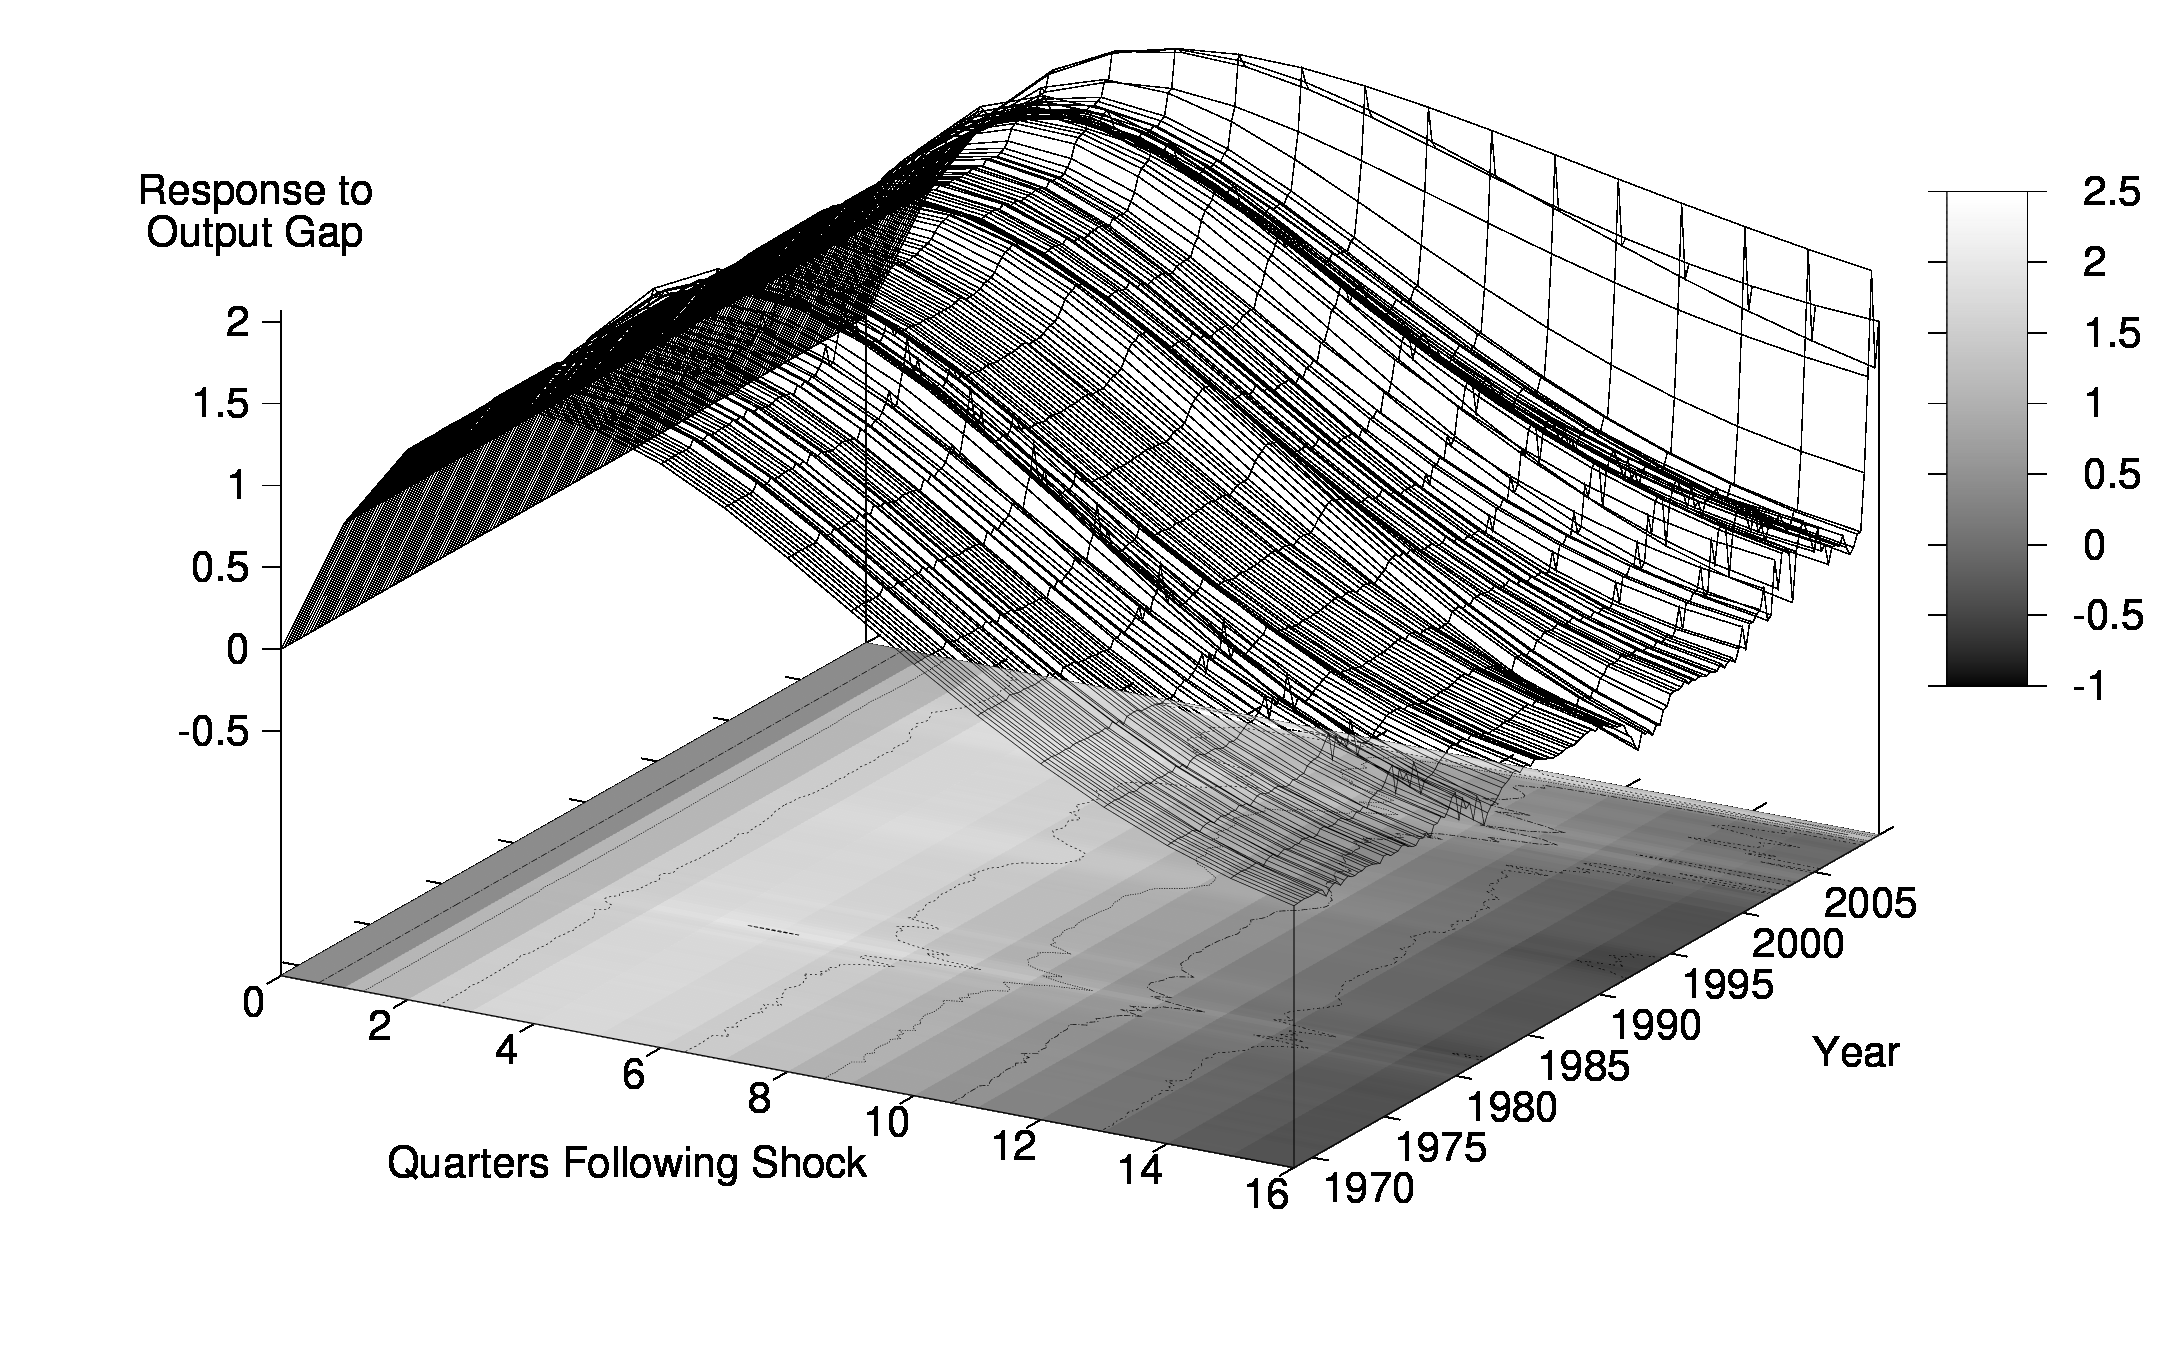
\includegraphics[scale=0.12]{images/Irf16_Output_Gap_Output_Judgment_Shock.png} & 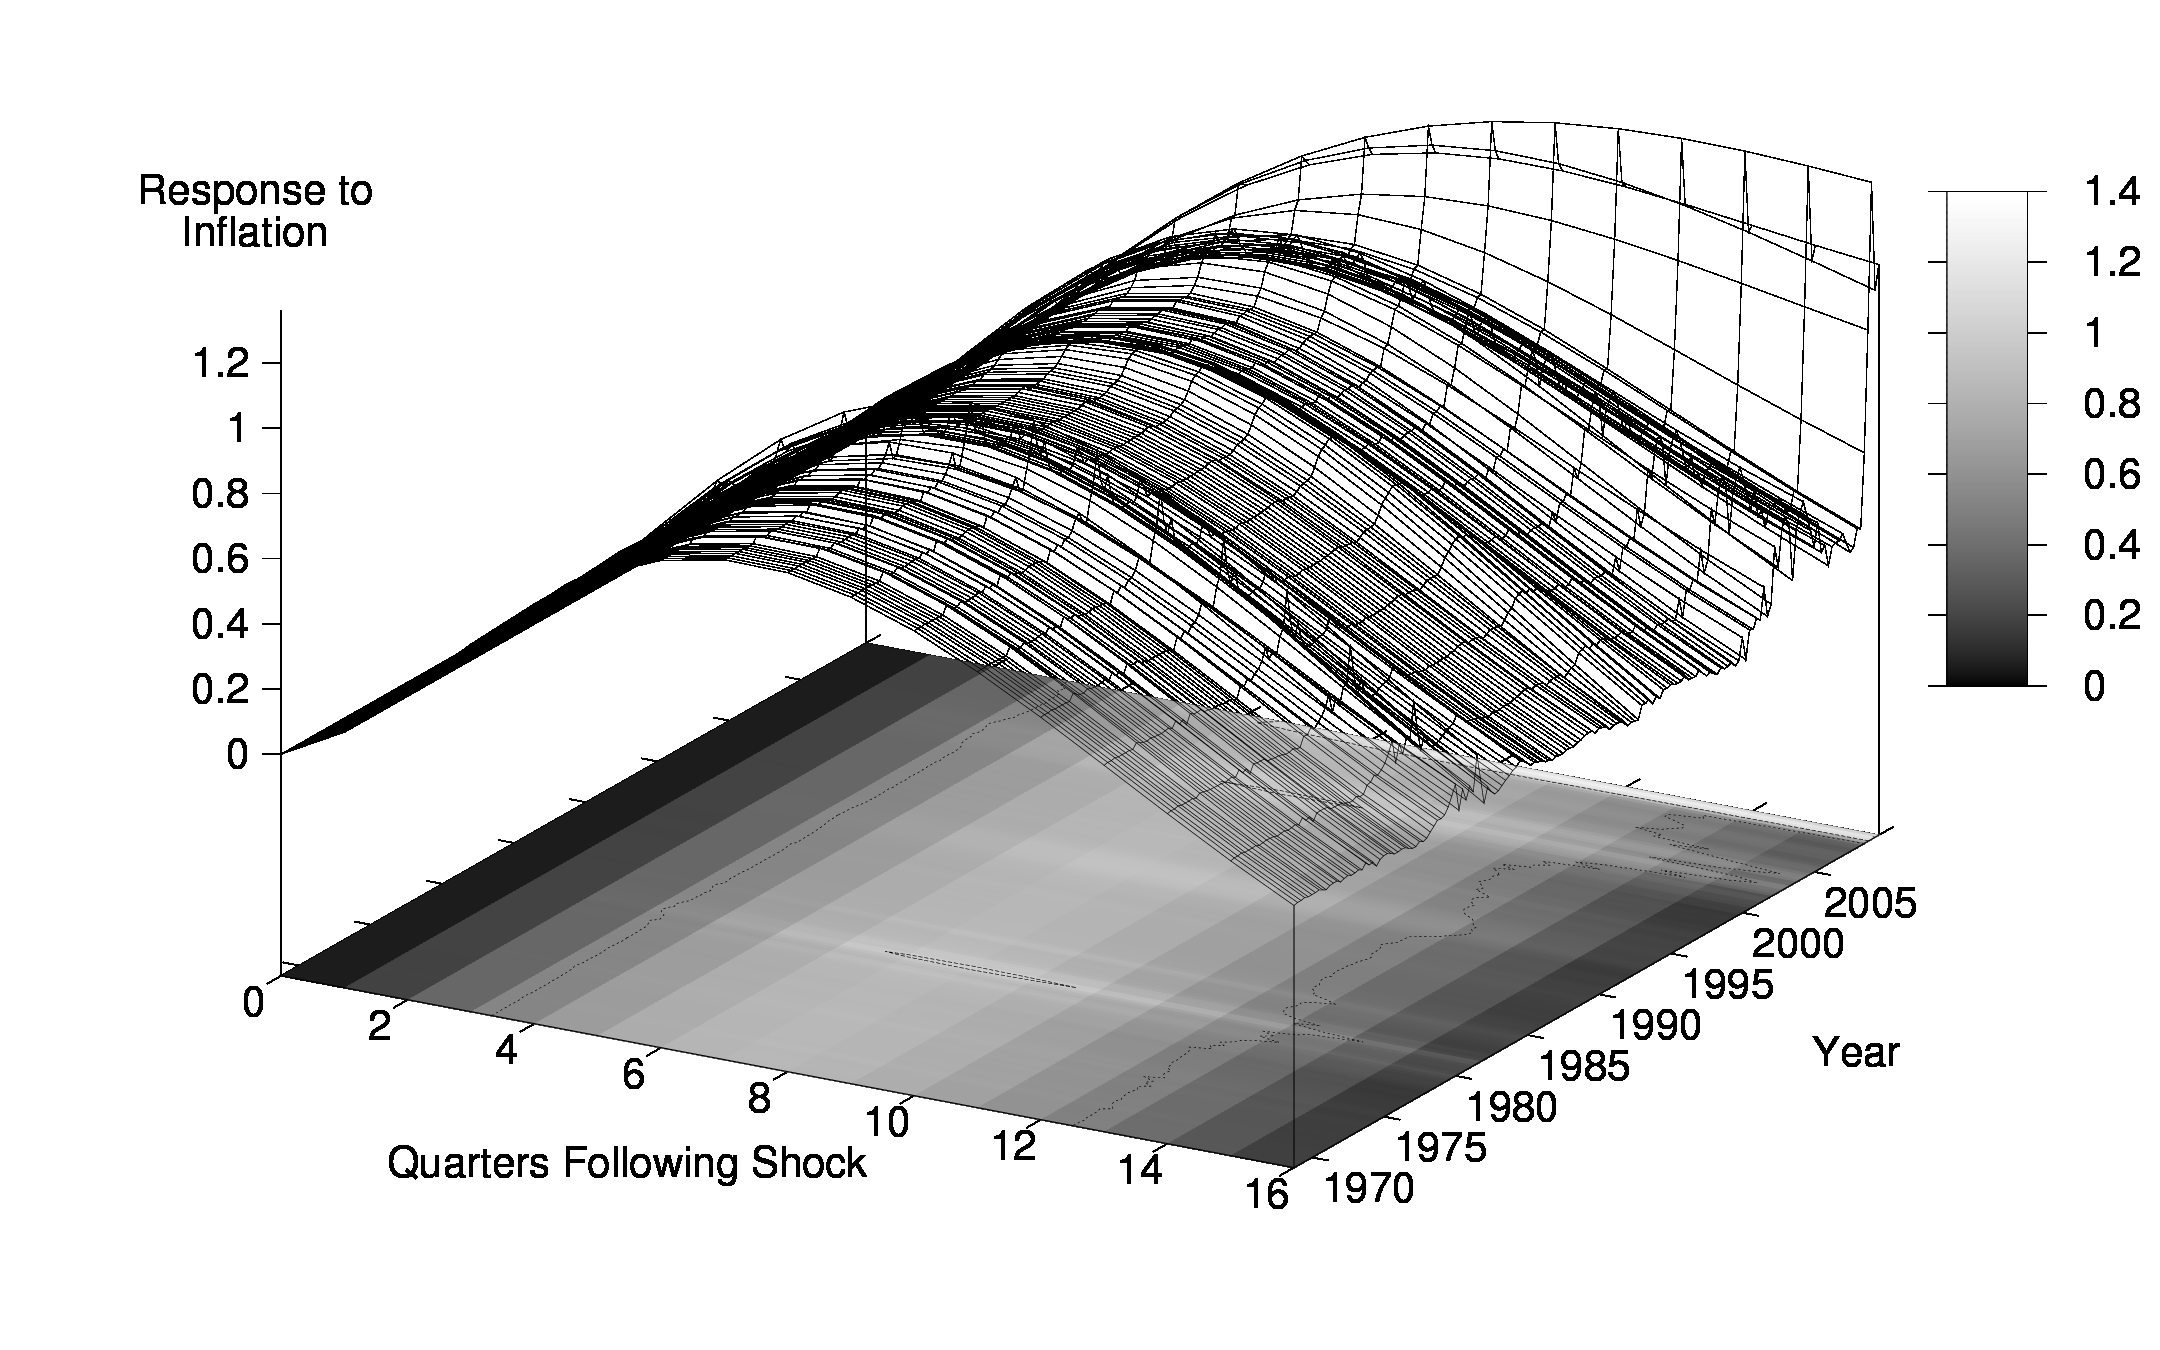
\includegraphics[scale=0.12]{images/Irf16_Inflation_Output_Judgment_Shock.png} \\\\
\textbf{Output Gap Response} & \textbf{Inflation Response} \\ 
\textbf{to Inflation Judgment Shock} & \textbf{to Inflation Judgment Shock}  \\
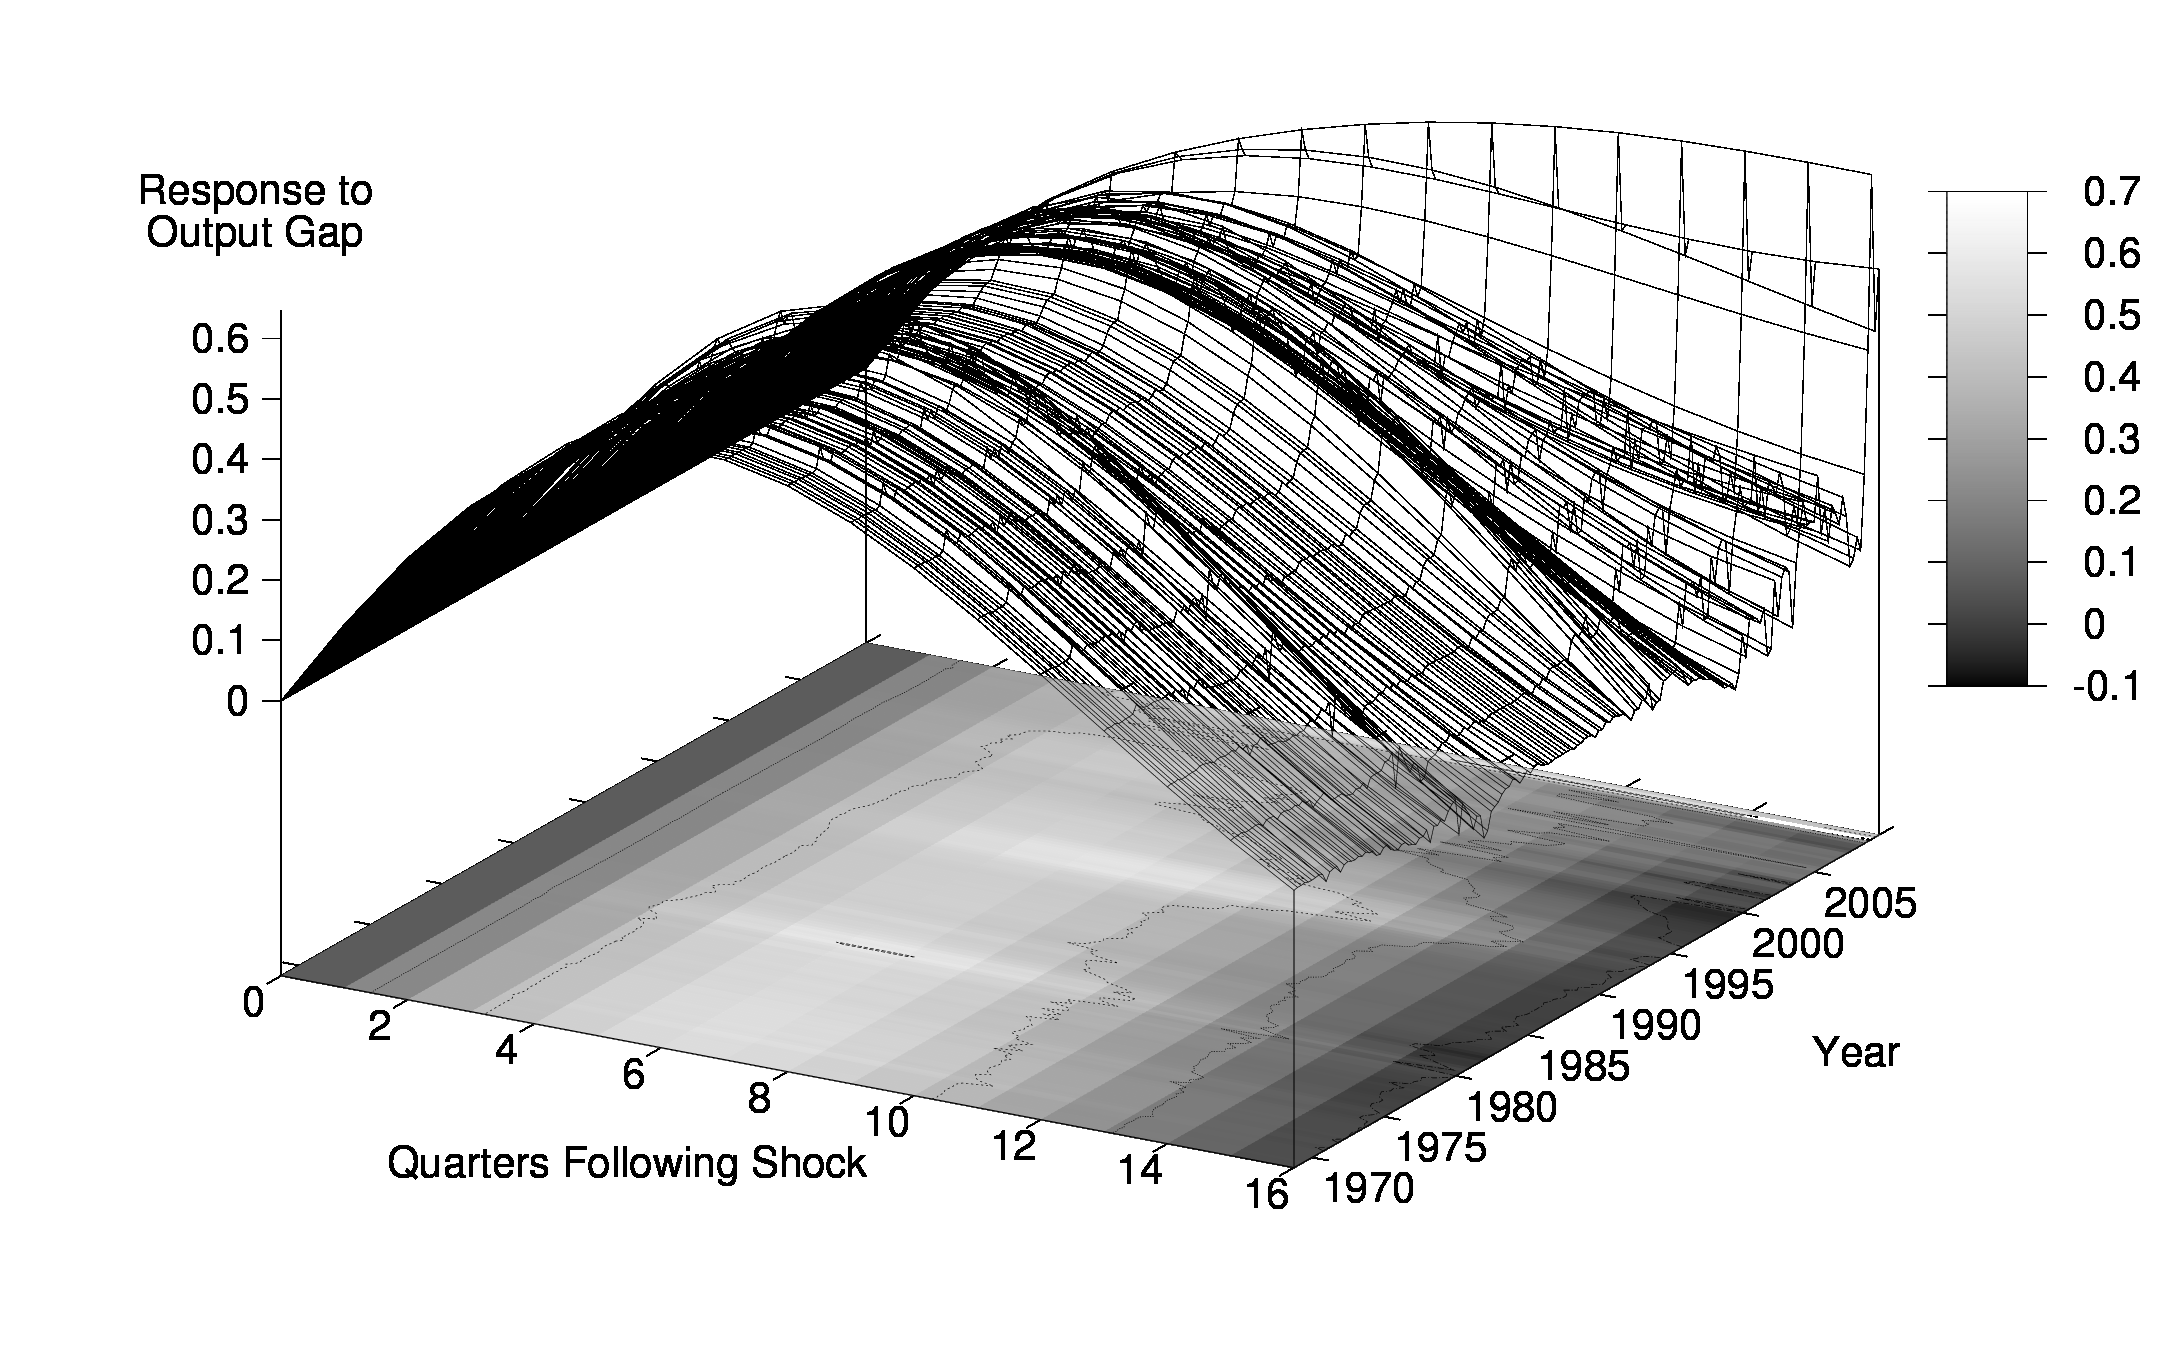
\includegraphics[scale=0.12]{images/Irf16_Output_Gap_Inflation_Judgment_Shock.png} & 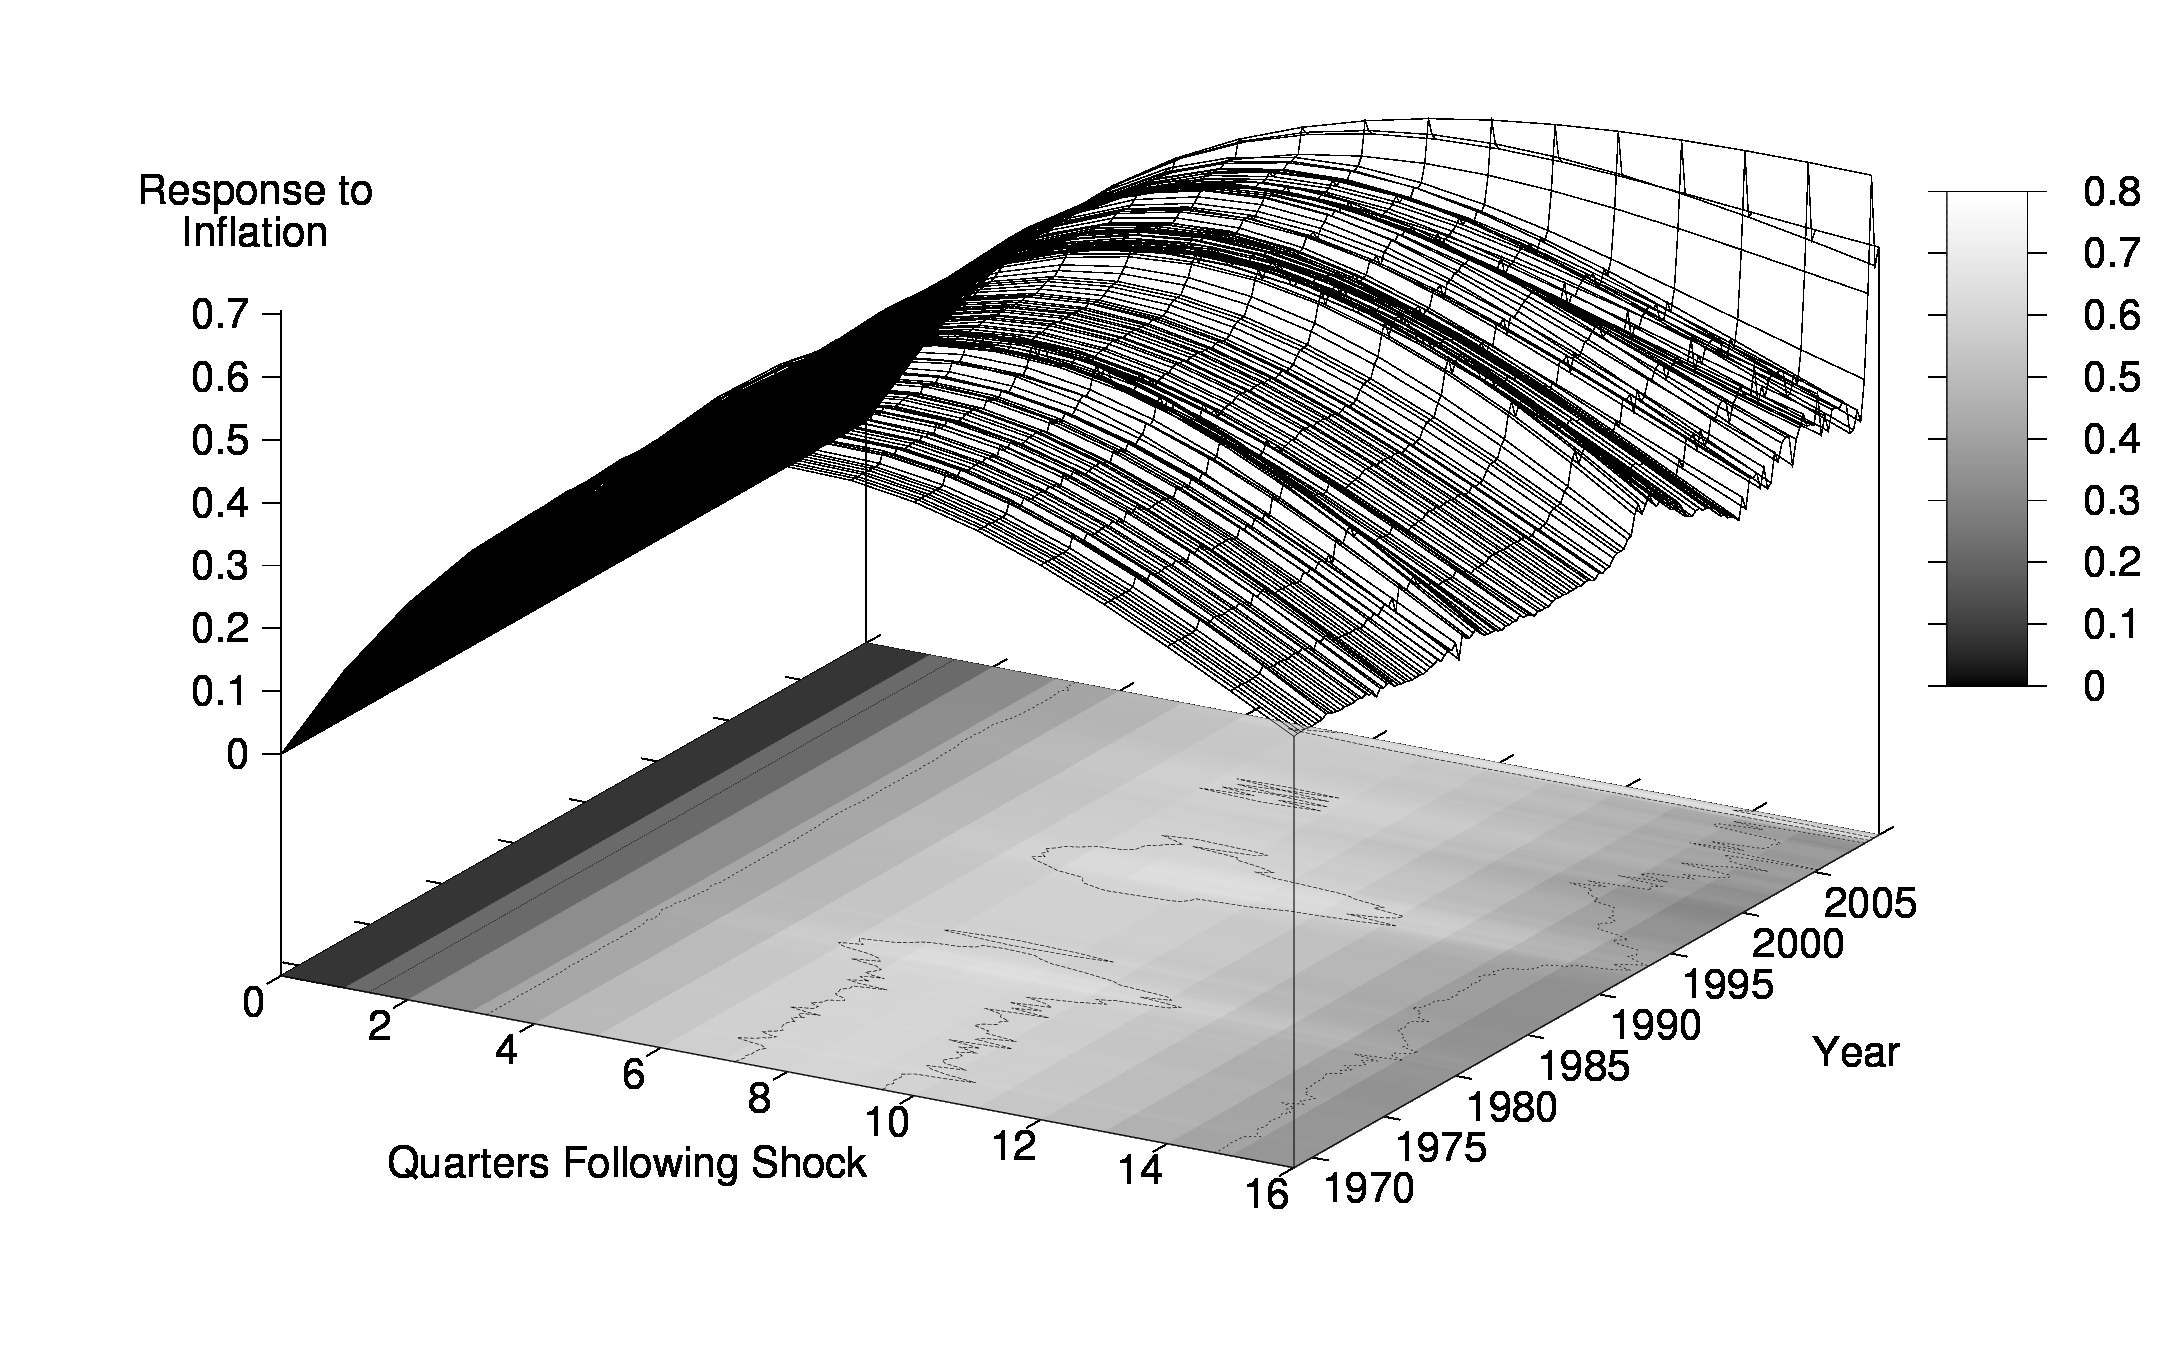
\includegraphics[scale=0.12]{images/Irf16_Inflation_Inflation_Judgment_Shock.png} \\
\end{tabular}
\end{figure}

\begin{figure}\caption{Root Mean Squared Response to Judgment Shocks}\label{fg:irf_judgment_size}
\hspace*{-2pc}
\begin{tabular}{cc}\\
\textbf{Output Gap Response} & \textbf{Inflation Response} \\
\textbf{to Output Judgment Shock} & \textbf{to Output Judgment Shock}  \\
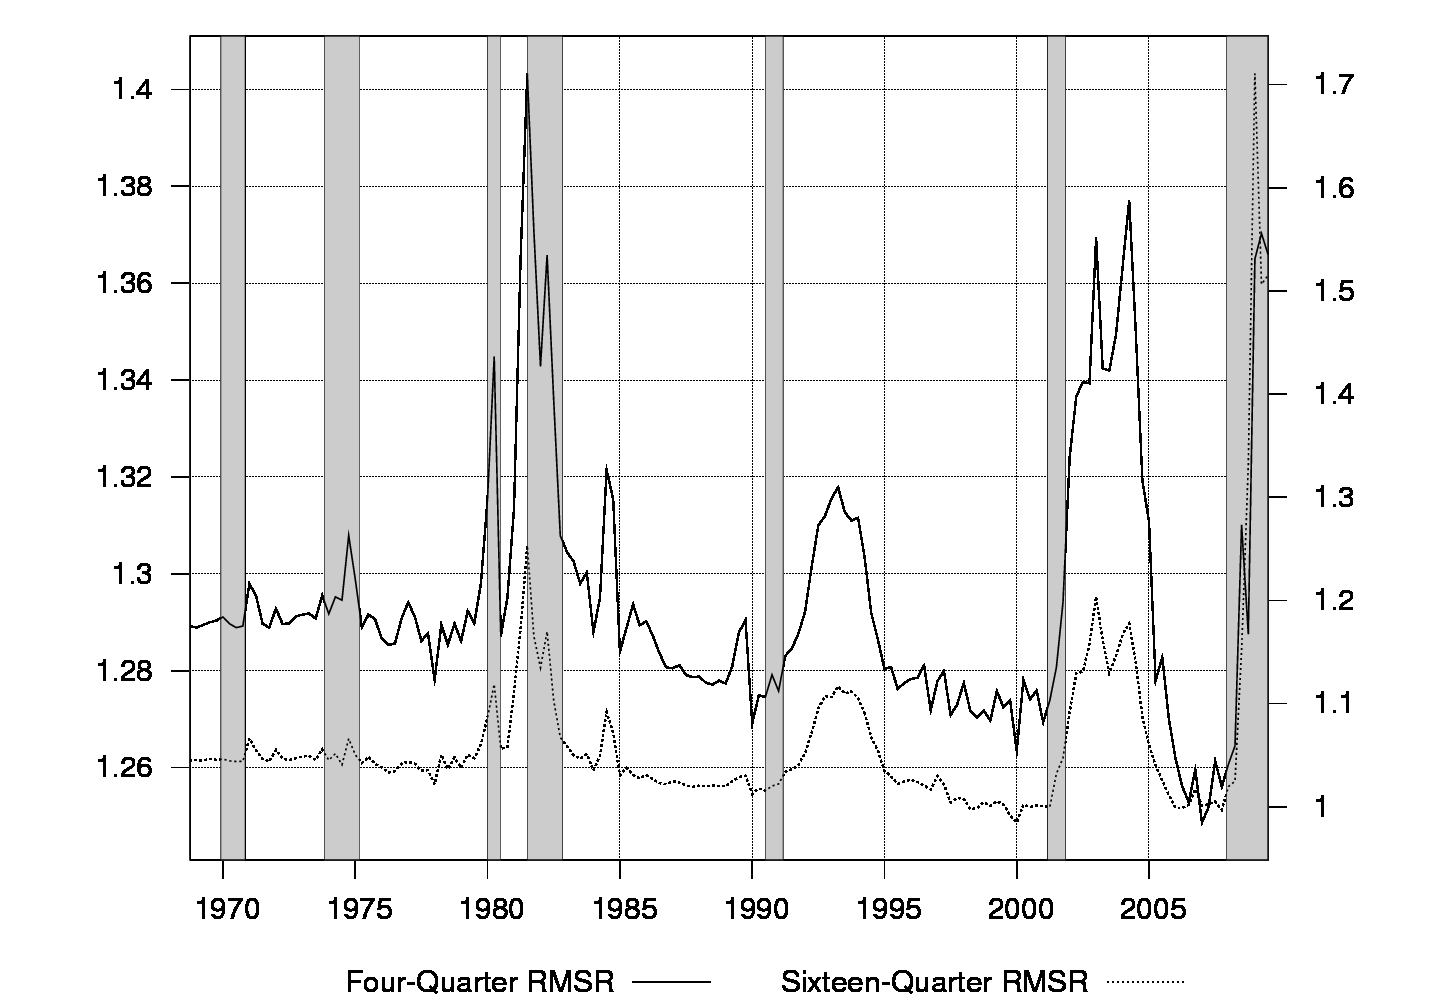
\includegraphics[scale=0.17]{images/RMS16_Output_Gap_Output_Judgment_Shock.png} & 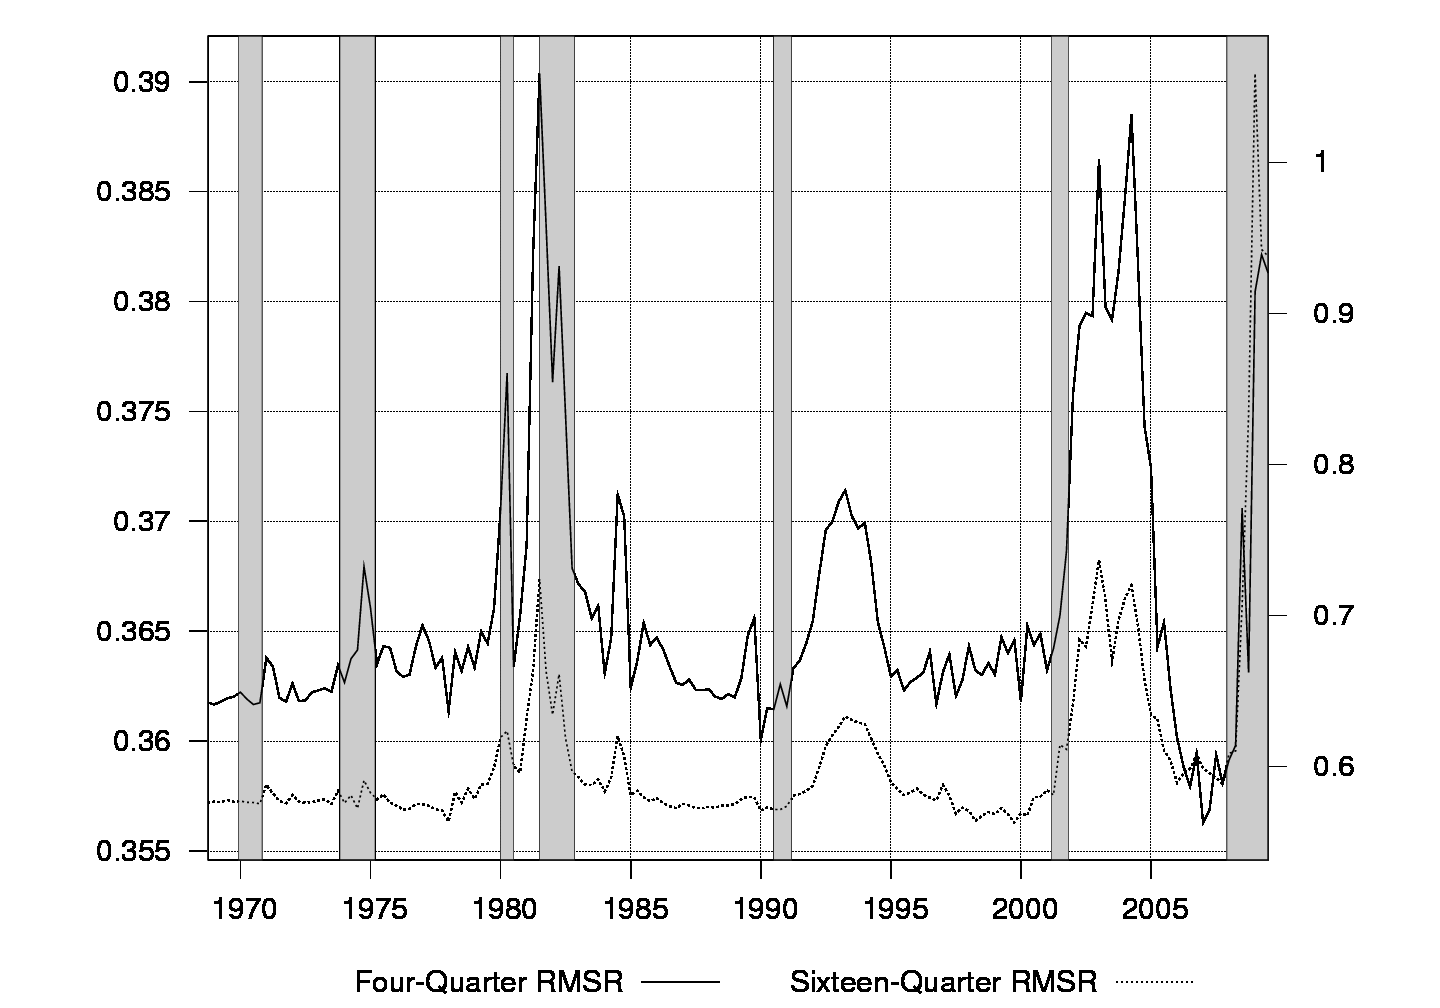
\includegraphics[scale=0.17]{images/RMS16_Inflation_Output_Judgment_Shock.png} \\\\
\textbf{Output Gap Response} & \textbf{Inflation Response} \\ 
\textbf{to Inflation Judgment Shock} & \textbf{to Inflation Judgment Shock}  \\
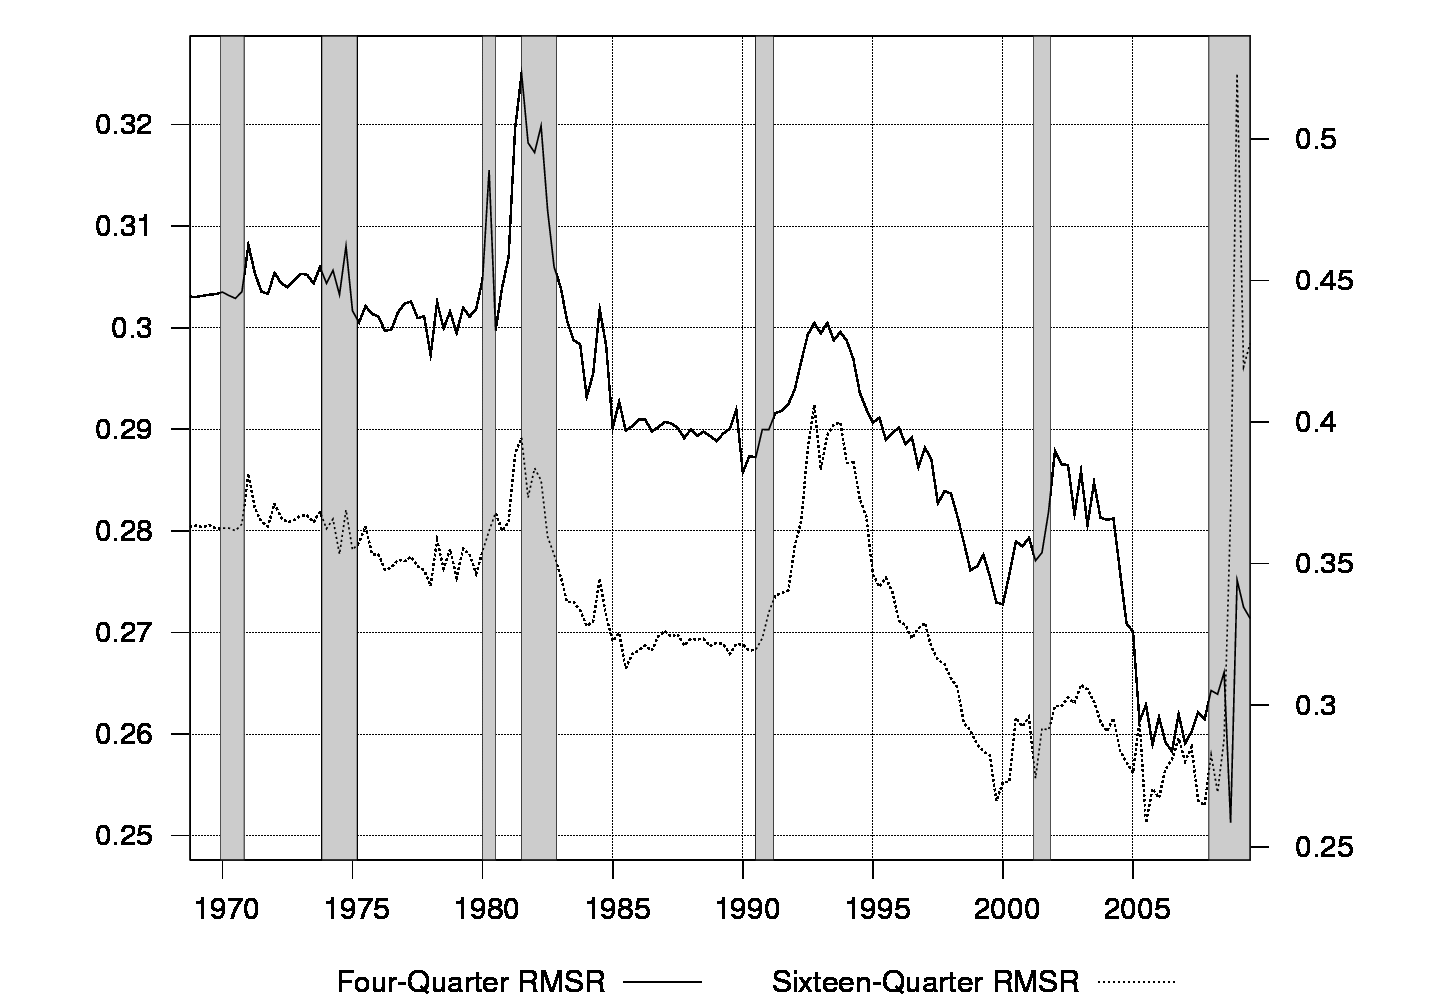
\includegraphics[scale=0.17]{images/RMS16_Output_Gap_Inflation_Judgment_Shock.png} & 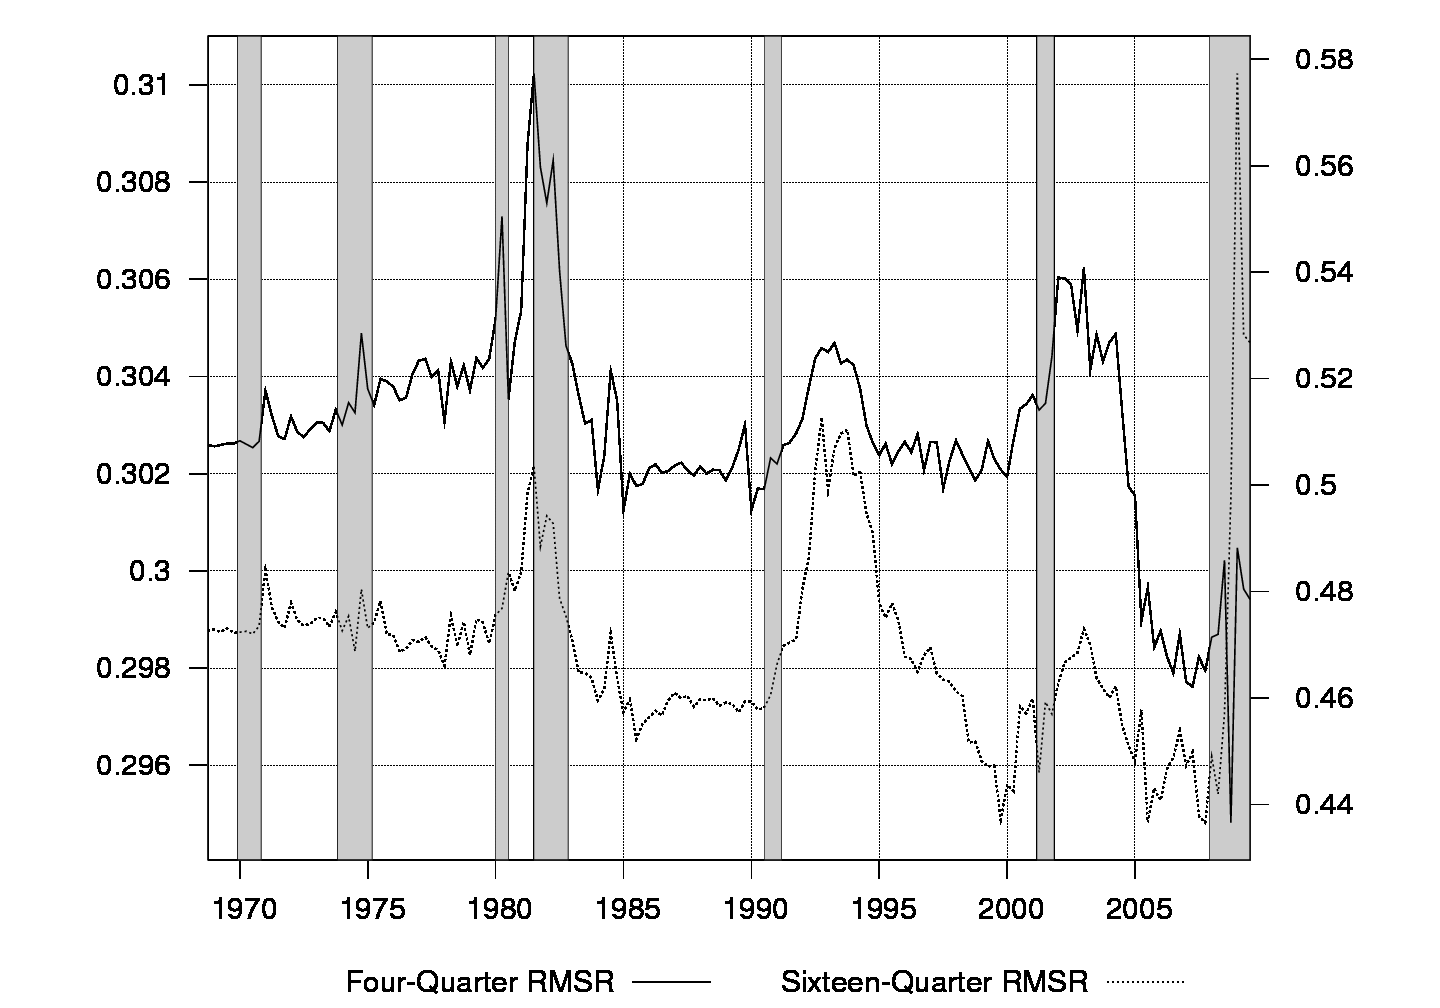
\includegraphics[scale=0.17]{images/RMS16_Inflation_Inflation_Judgment_Shock.png} \\
\end{tabular}
\end{figure}

\begin{figure}\caption{Impulse Response Functions: Structural Shocks}\label{fg:irf_structural}
\hspace*{-4pc}
\begin{tabular}{cc}\\
\textbf{Output Gap Response} & \textbf{Inflation Response} \\
\textbf{to Natural Rate Shock} & \textbf{to Natural Rate Shock}  \\
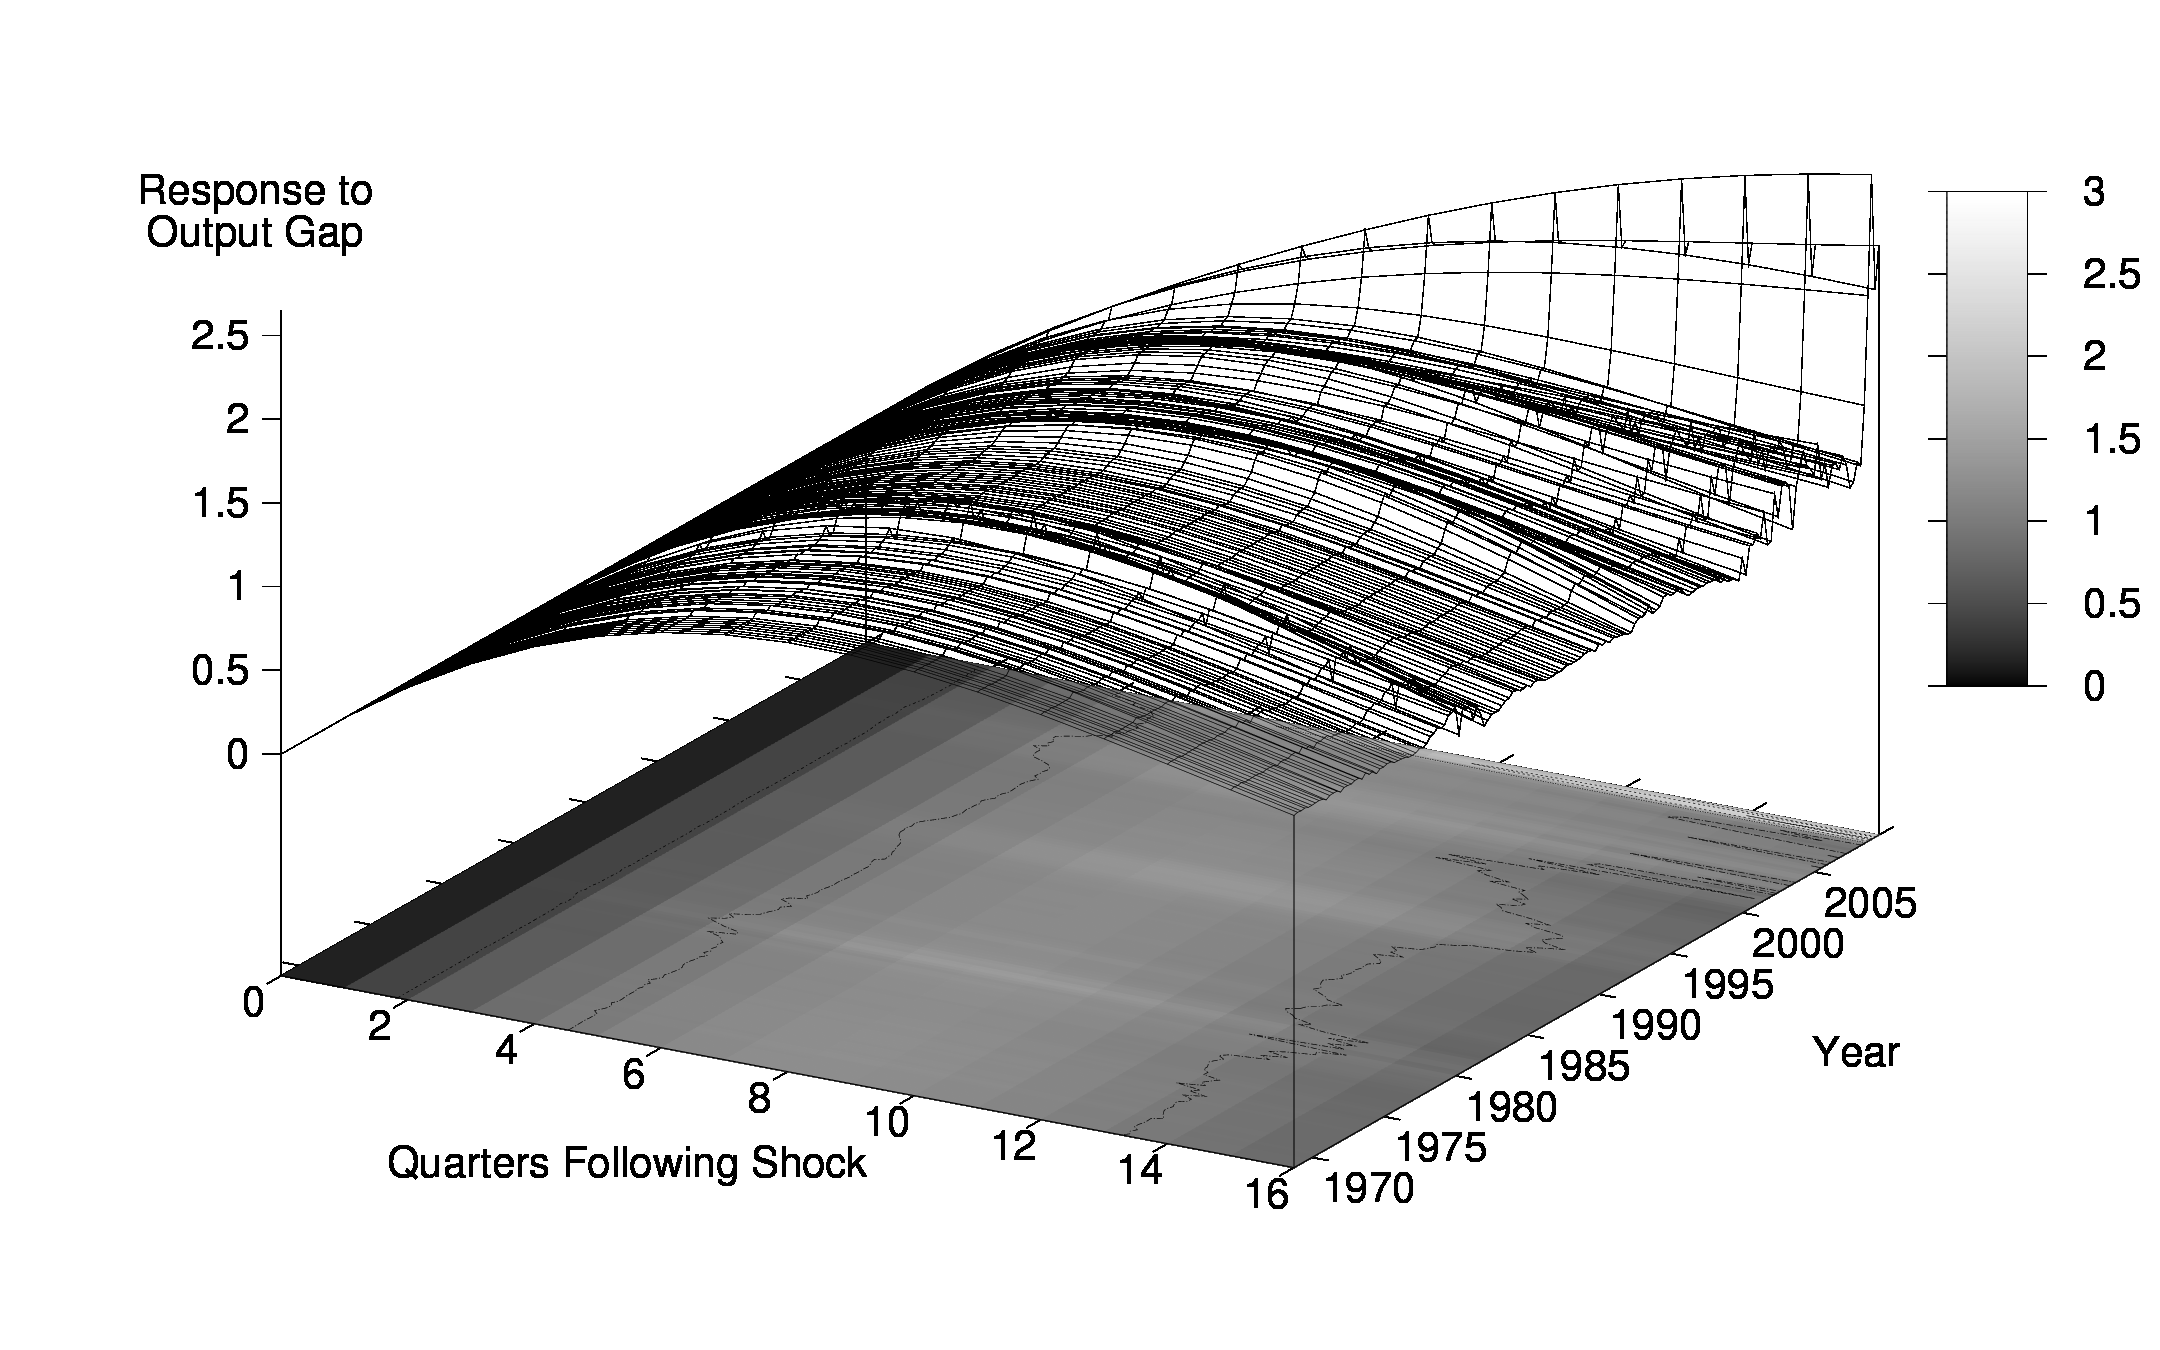
\includegraphics[scale=0.12]{images/Irf16_Output_Gap_Natural_Rate_Shock.png} & 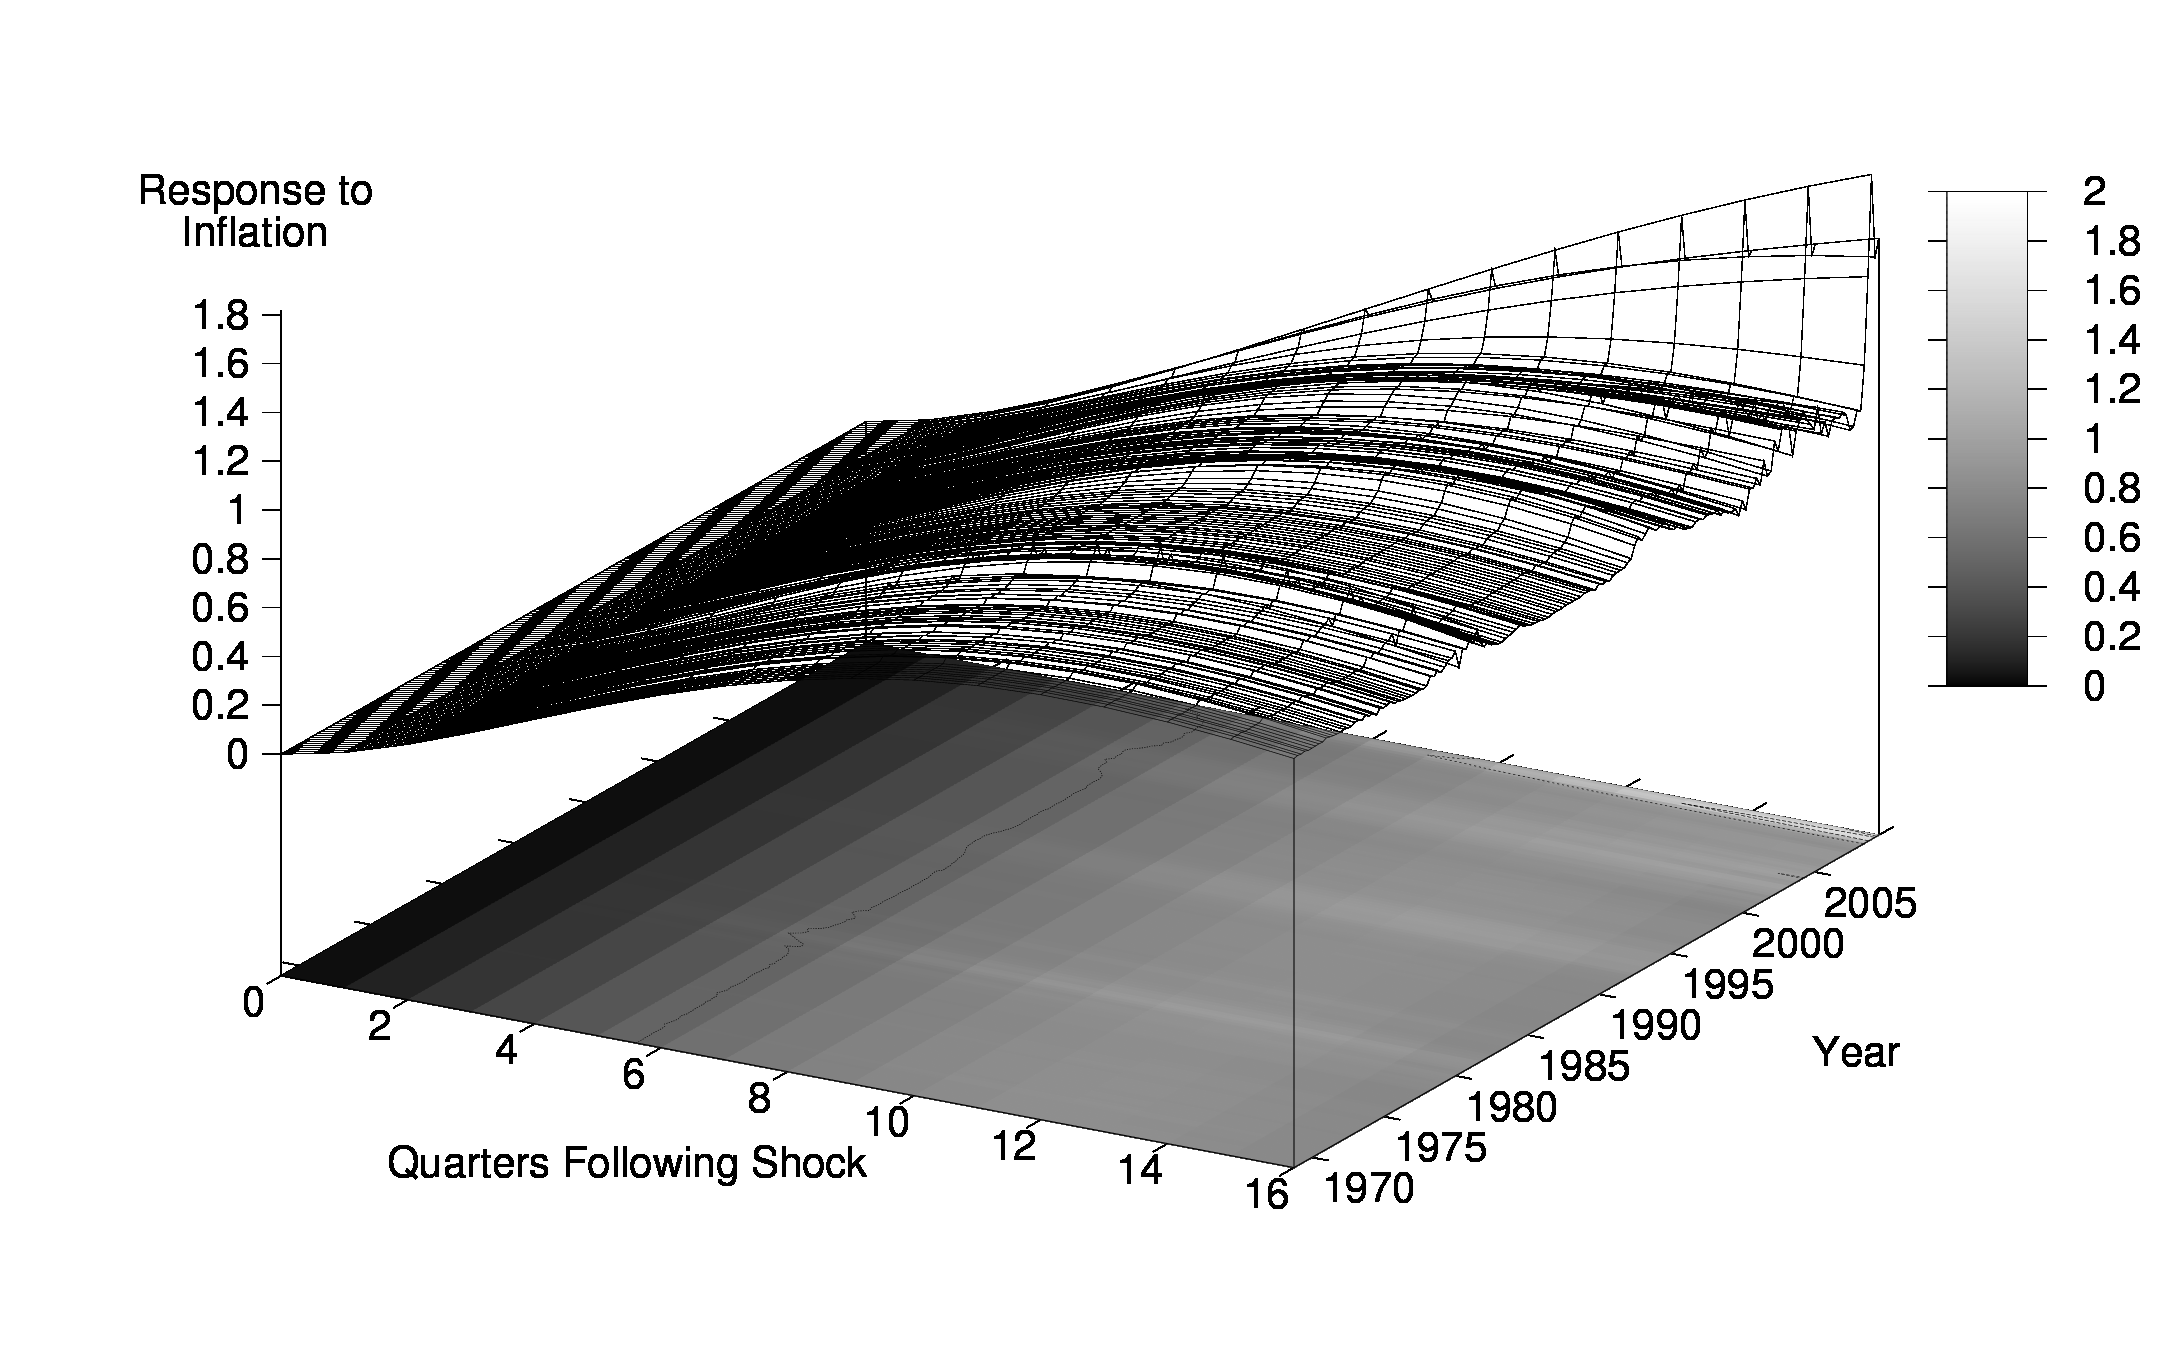
\includegraphics[scale=0.12]{images/Irf16_Inflation_Natural_Rate_Shock.png} \\\\
\textbf{Output Gap Response} & \textbf{Inflation Response} \\
\textbf{to Cost Shock} & \textbf{to Cost Shock}  \\
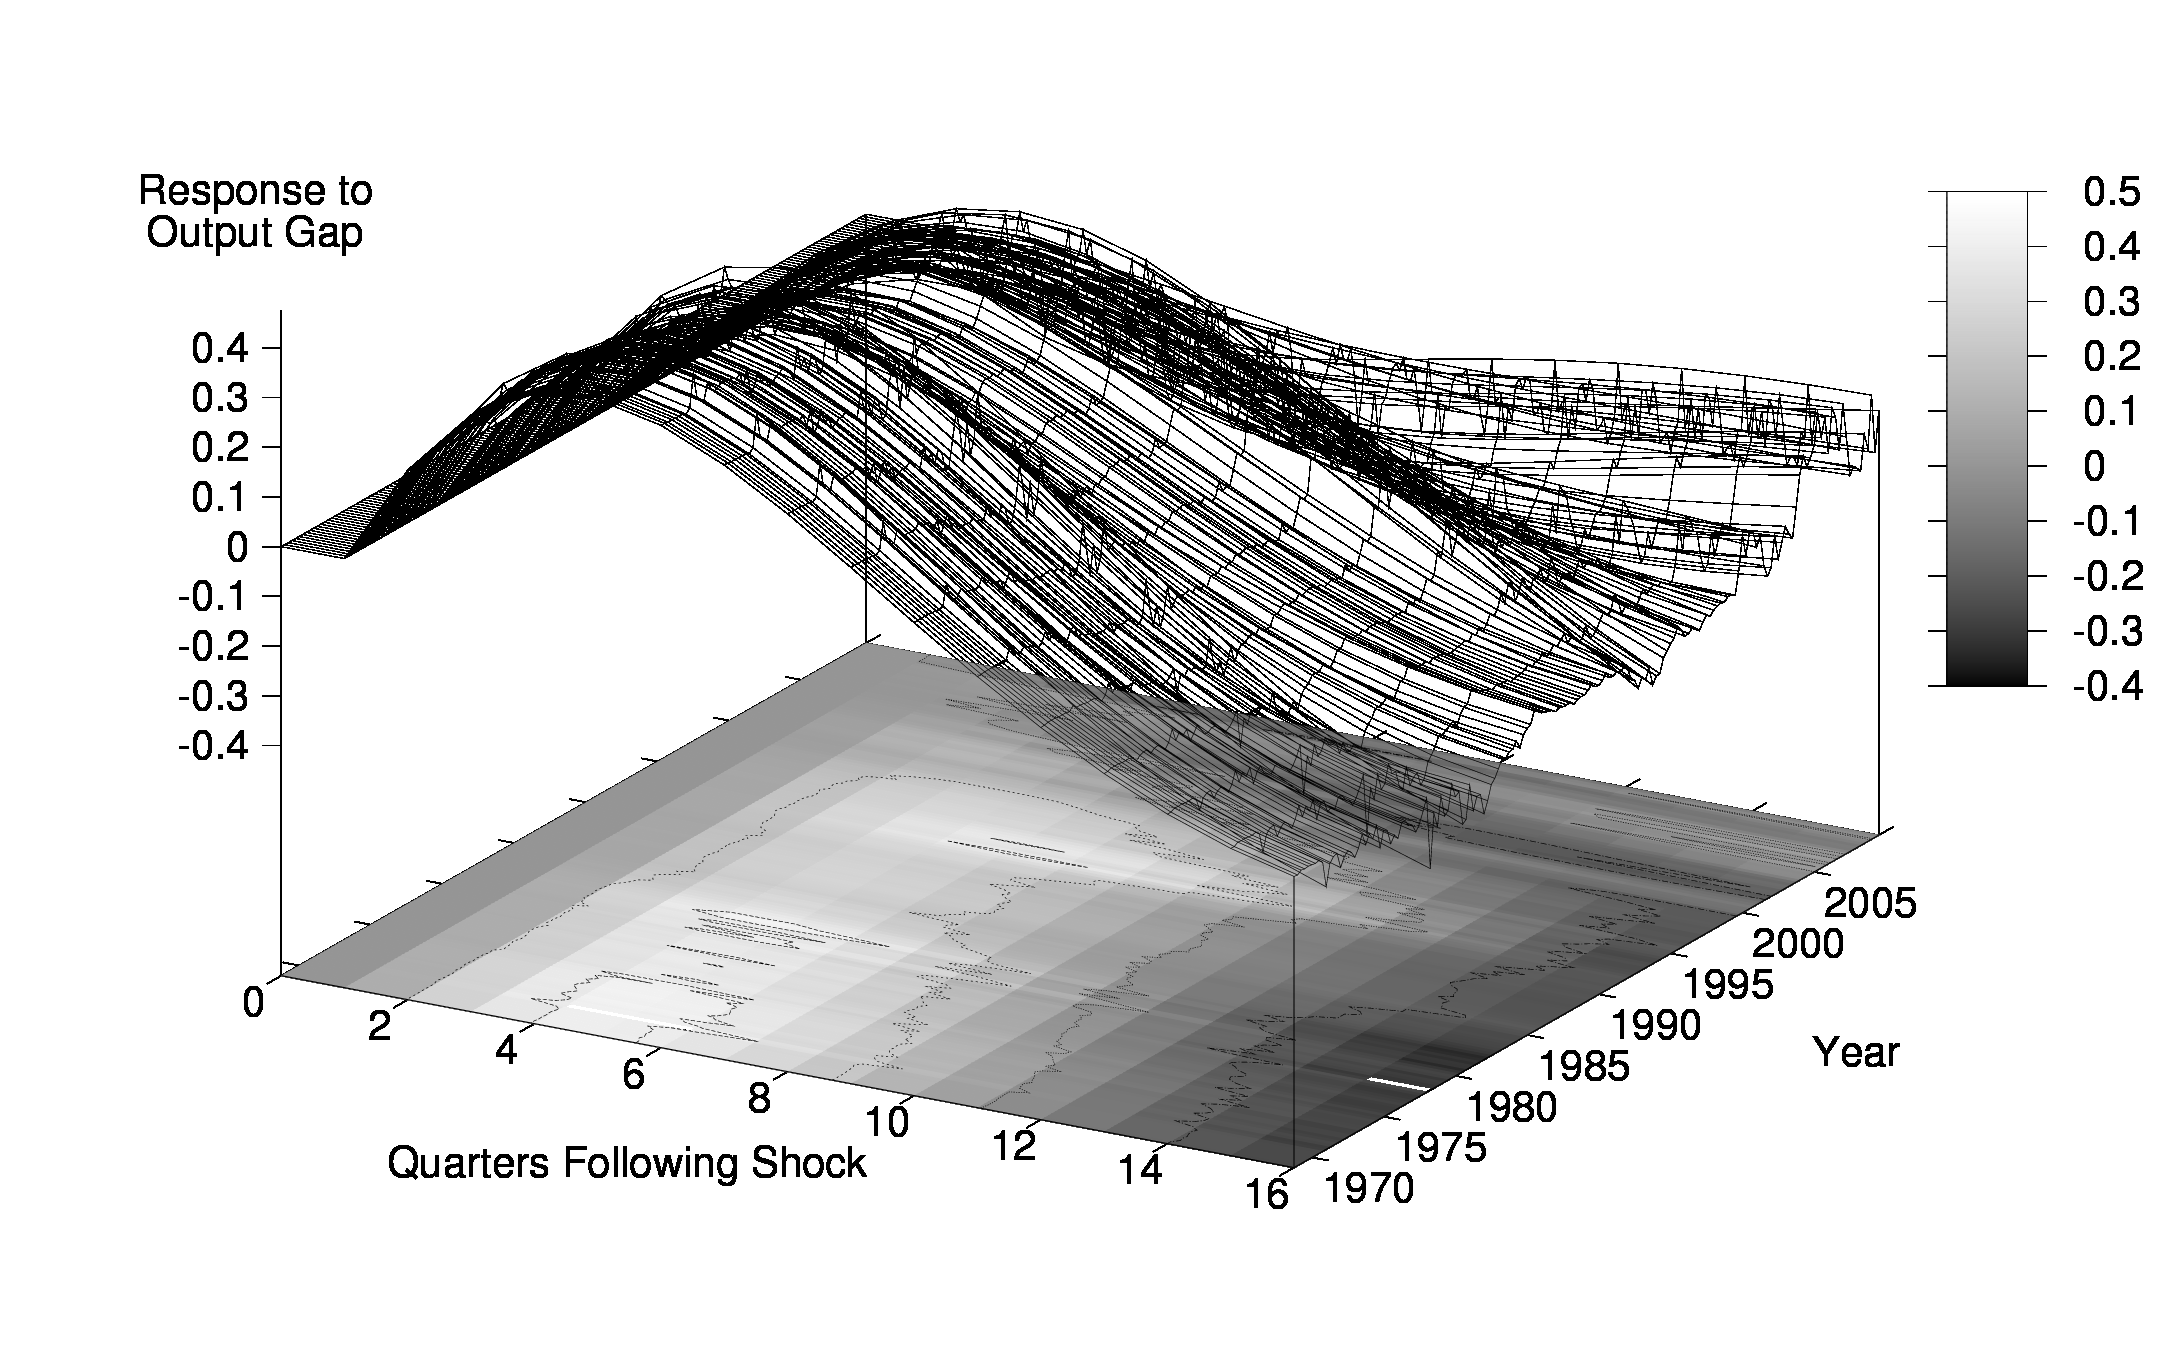
\includegraphics[scale=0.12]{images/Irf16_Output_Gap_Cost_Shock.png} & 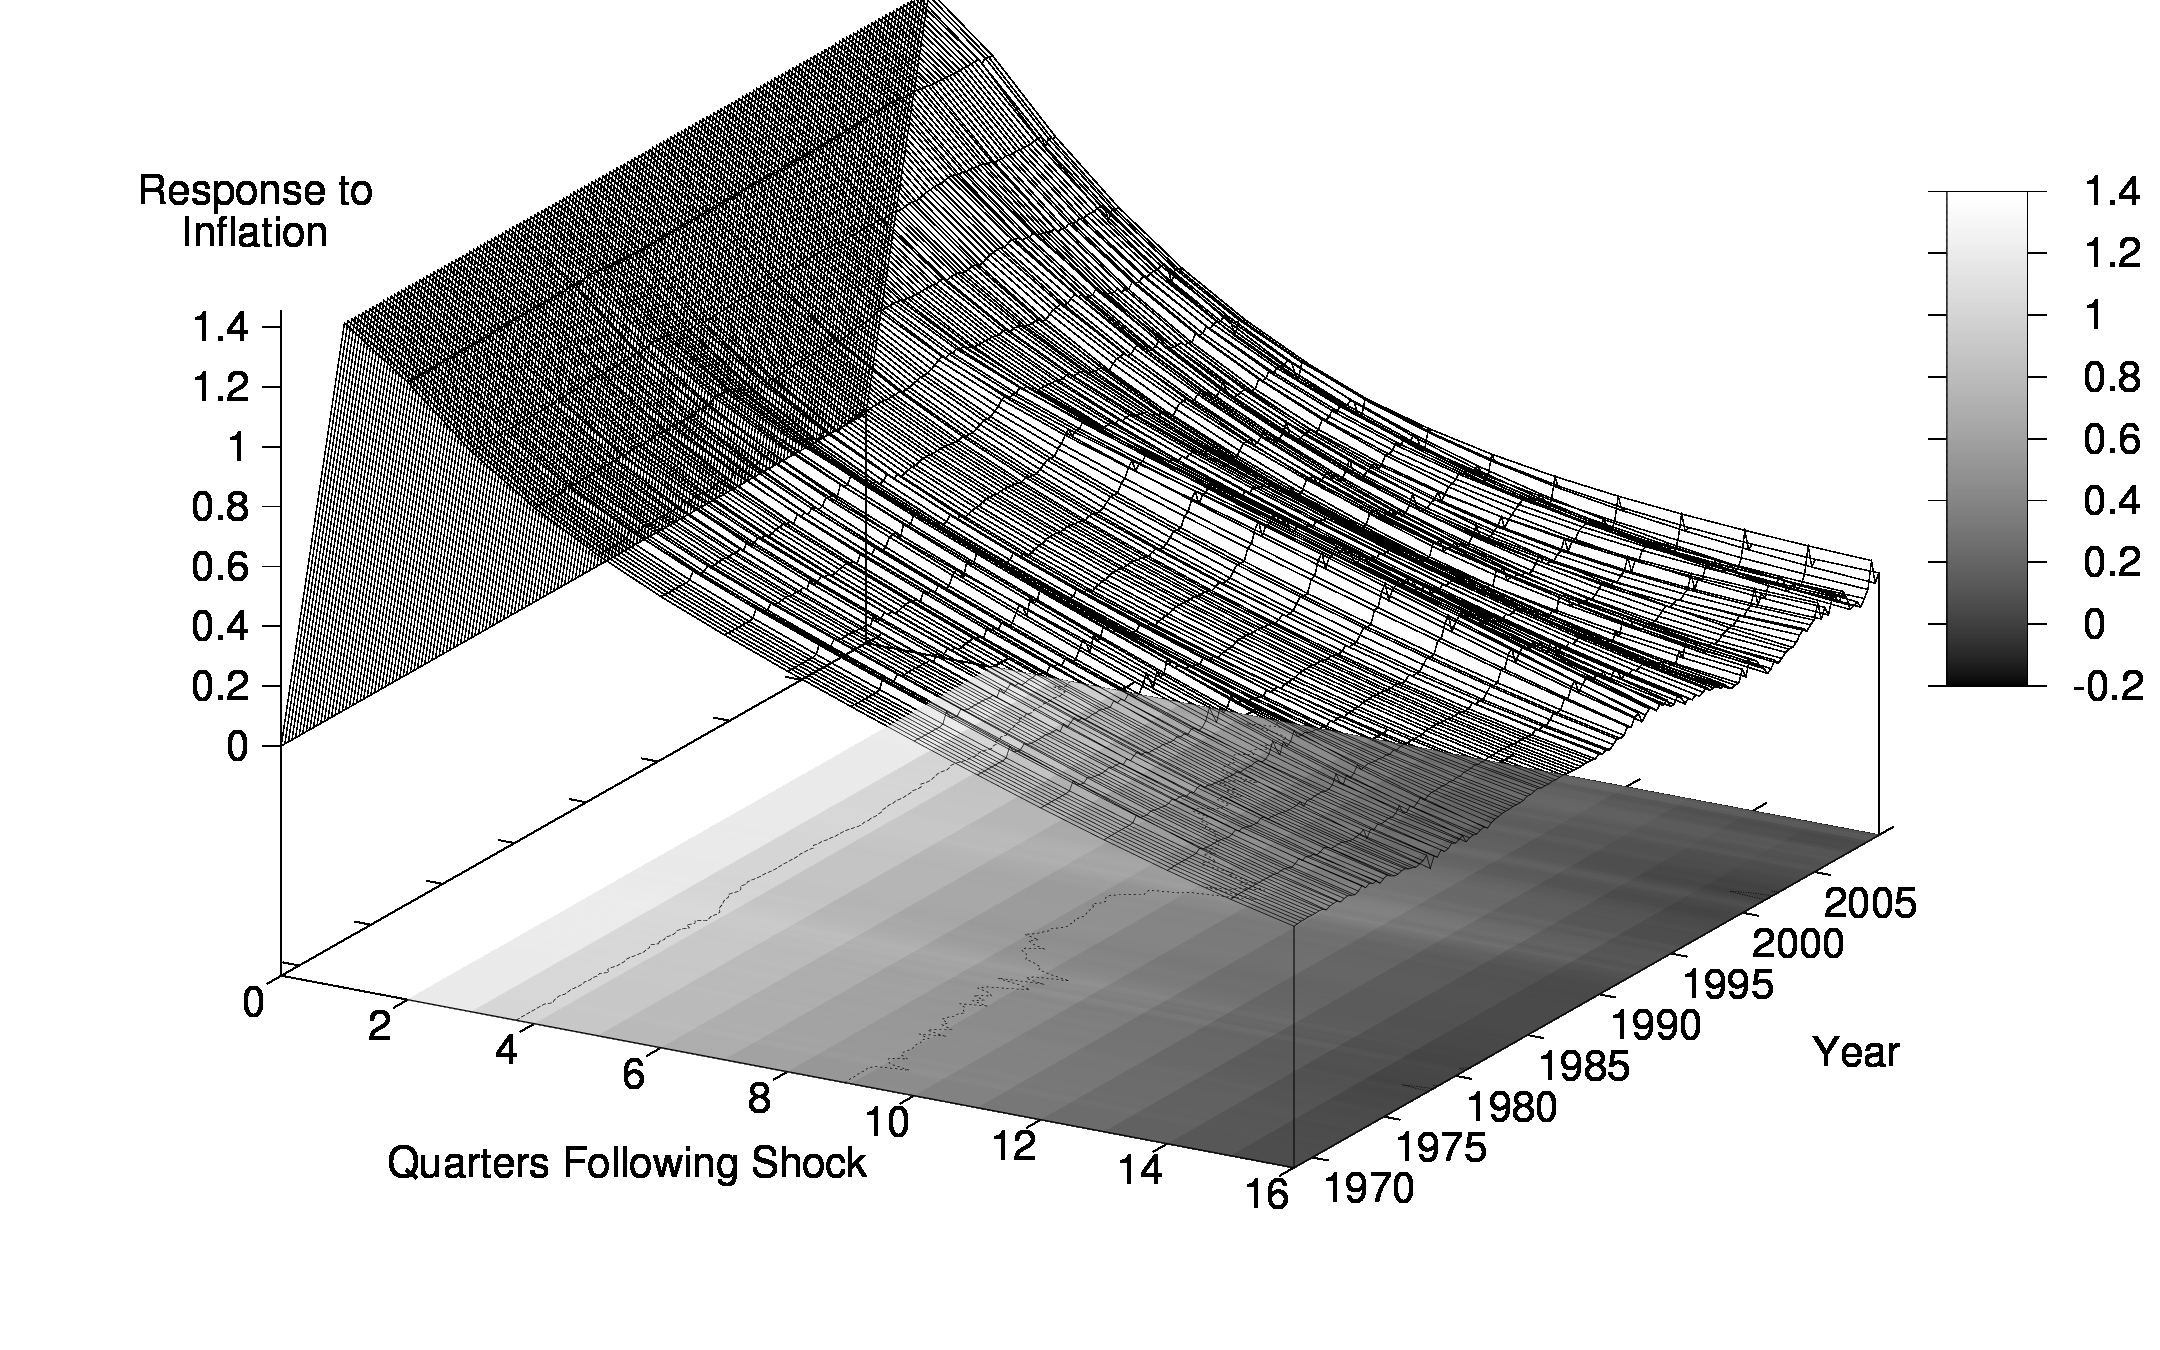
\includegraphics[scale=0.12]{images/Irf16_Inflation_Cost_Shock.png} \\\\
\textbf{Output Gap Response} & \textbf{Inflation Response} \\
\textbf{to Monetary Policy Shock} & \textbf{to Monetary Policy Shock}  \\
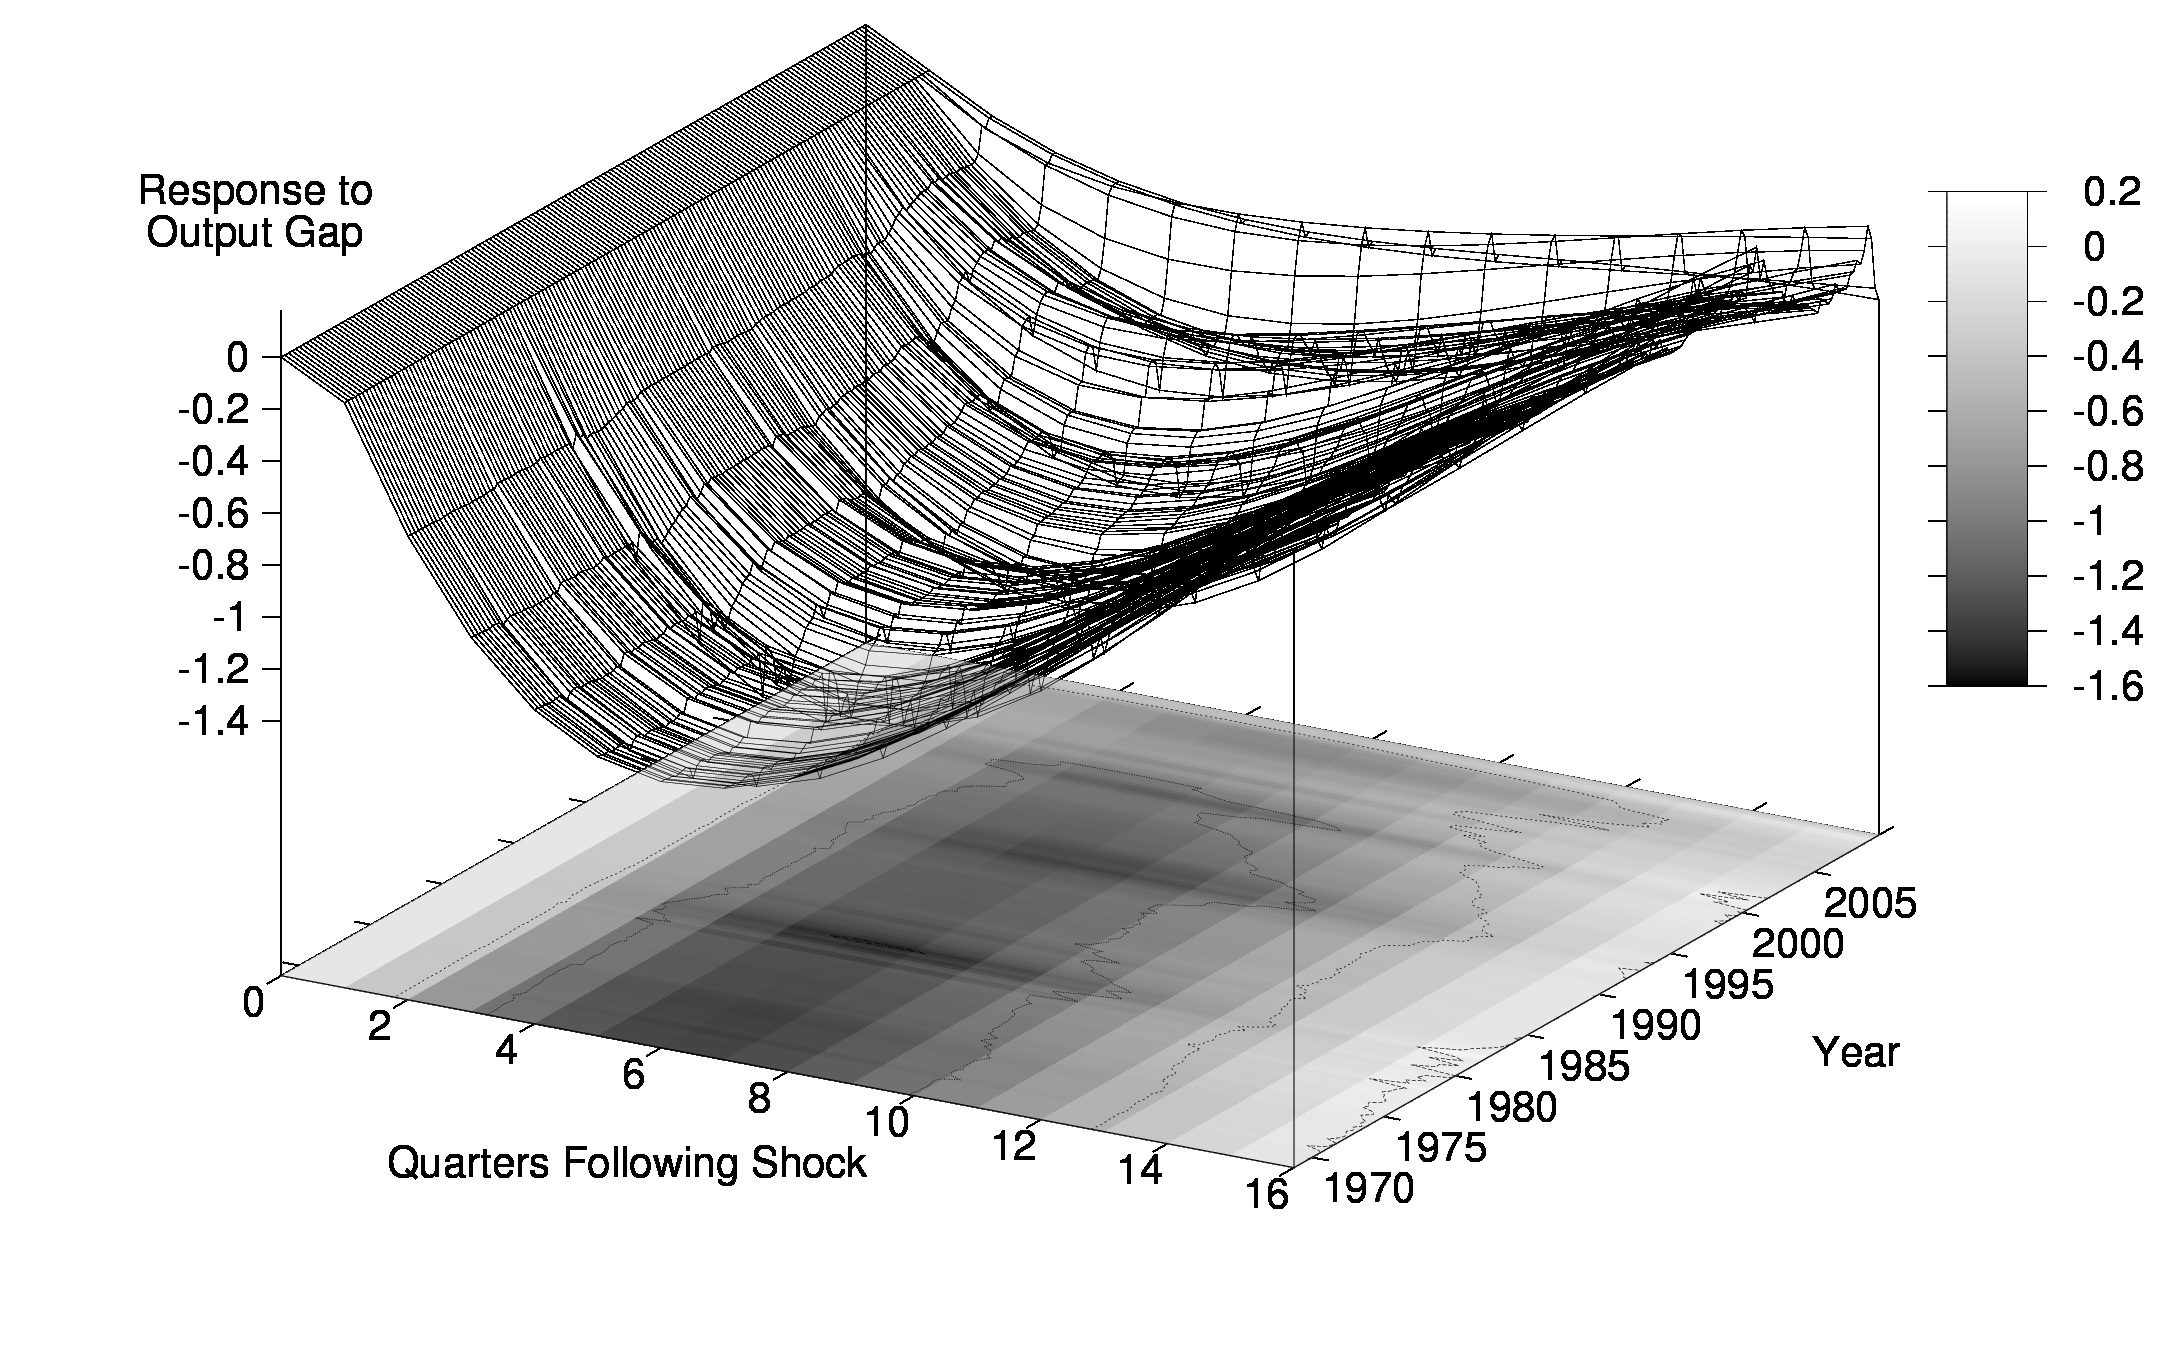
\includegraphics[scale=0.12]{images/Irf16_Output_Gap_Monetary_Policy_Shock.png} & 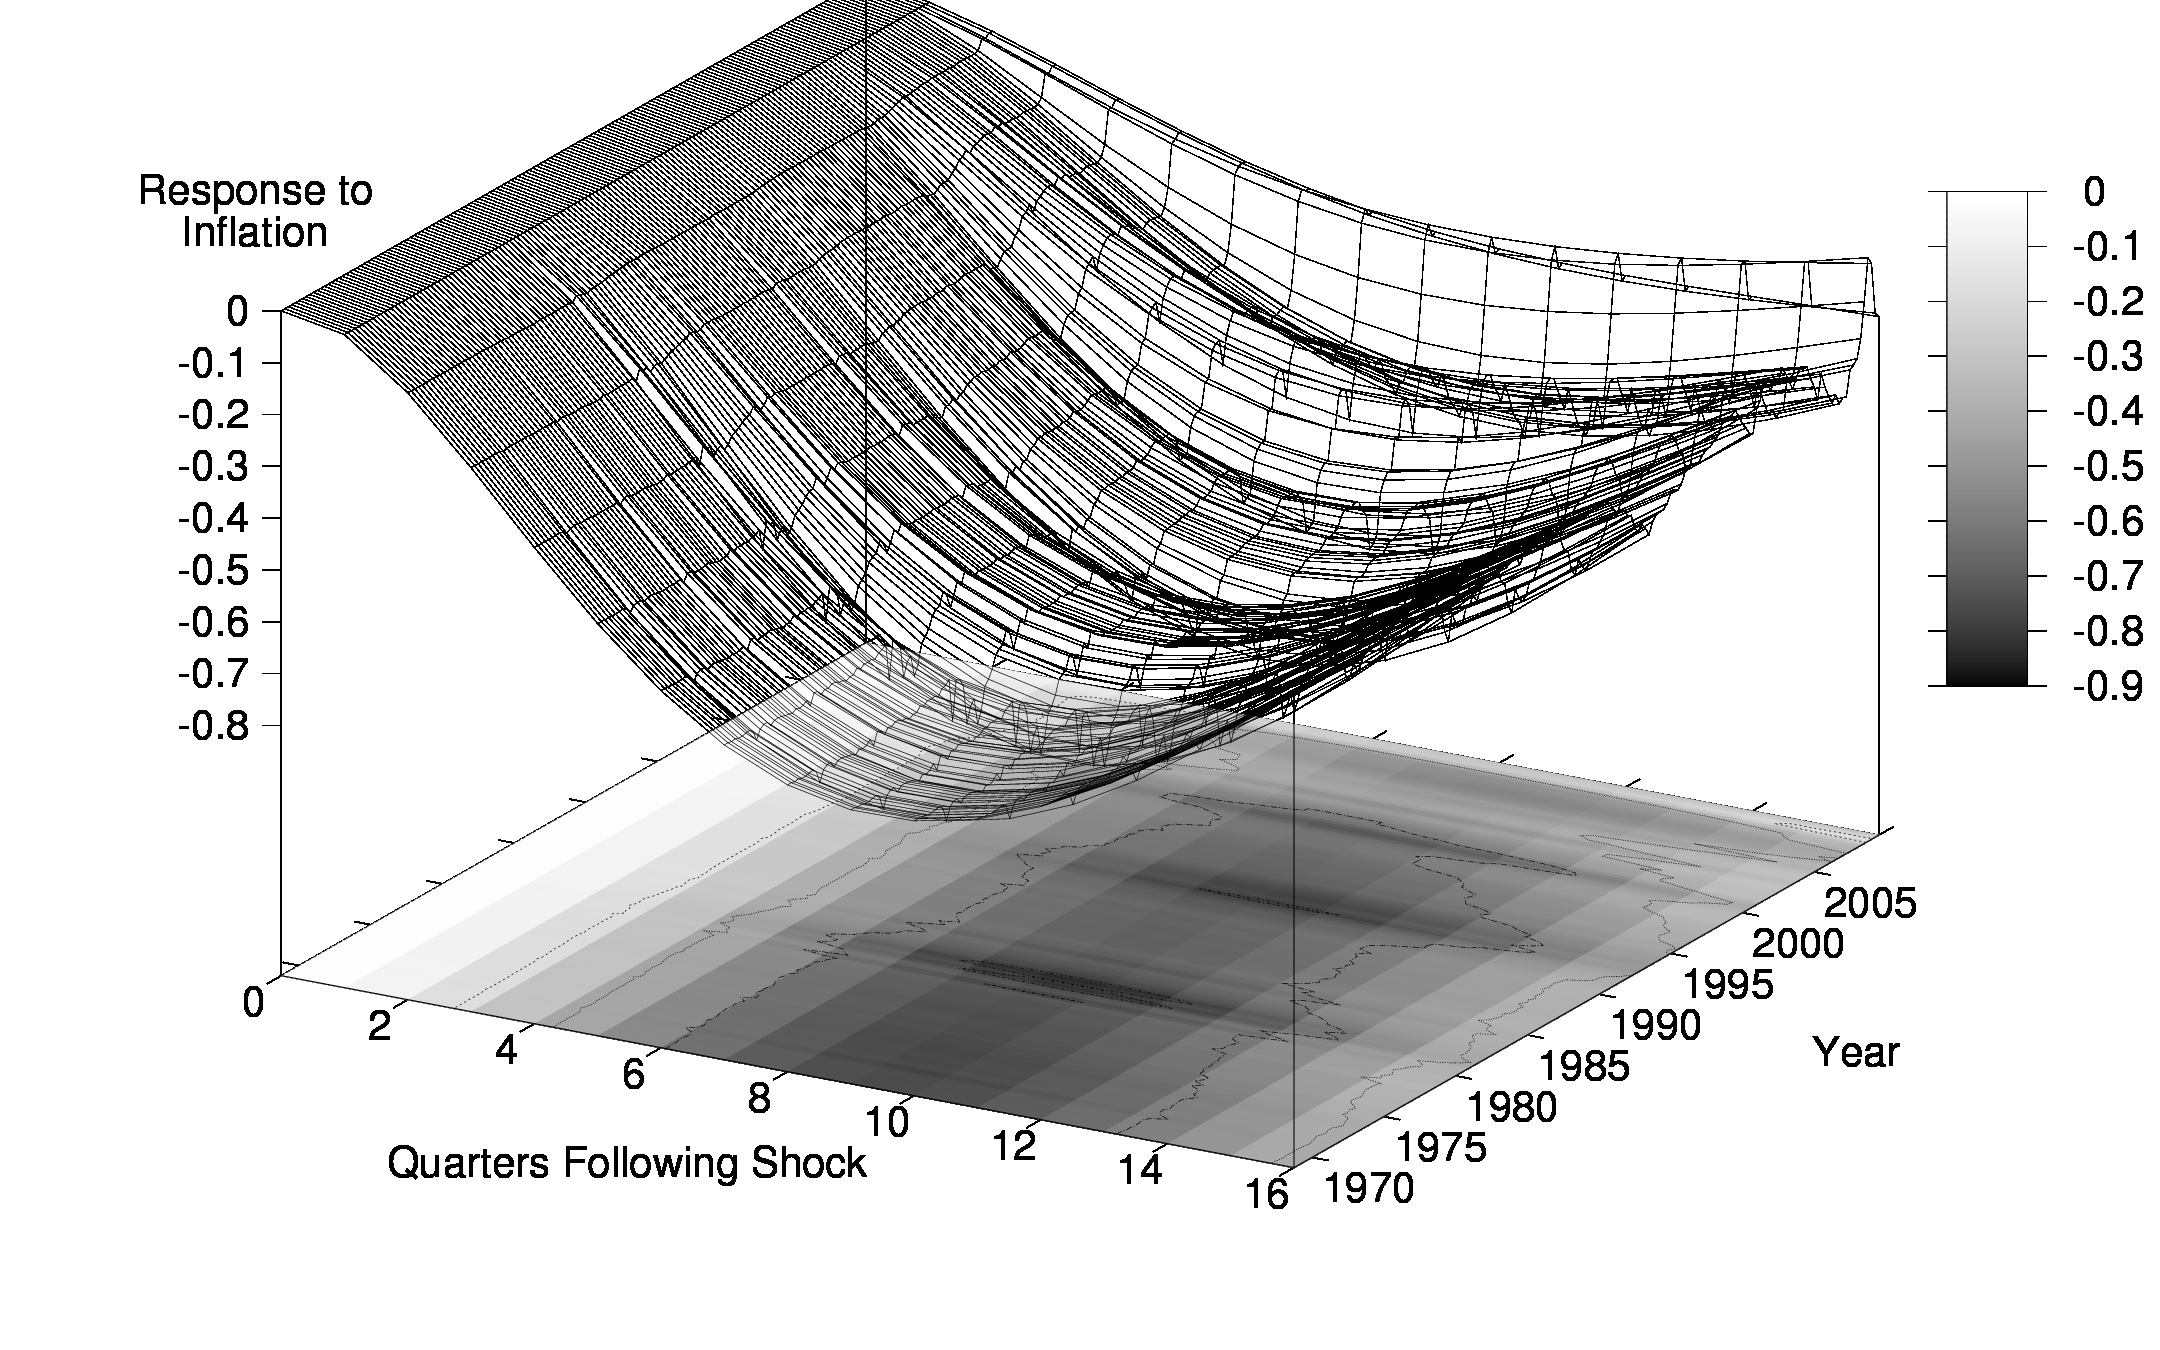
\includegraphics[scale=0.12]{images/Irf16_Inflation_Monetary_Policy_Shock.png} 
\end{tabular}
\end{figure}

\begin{figure}\caption{Root Mean Squared Response Structural Shocks}\label{fg:irf_structural_size}
\hspace*{-2pc}
\begin{tabular}{cc}\\
\textbf{Output Gap Response} & \textbf{Inflation Response} \\
\textbf{to Natural Rate Shock} & \textbf{to Natural Rate Shock}  \\
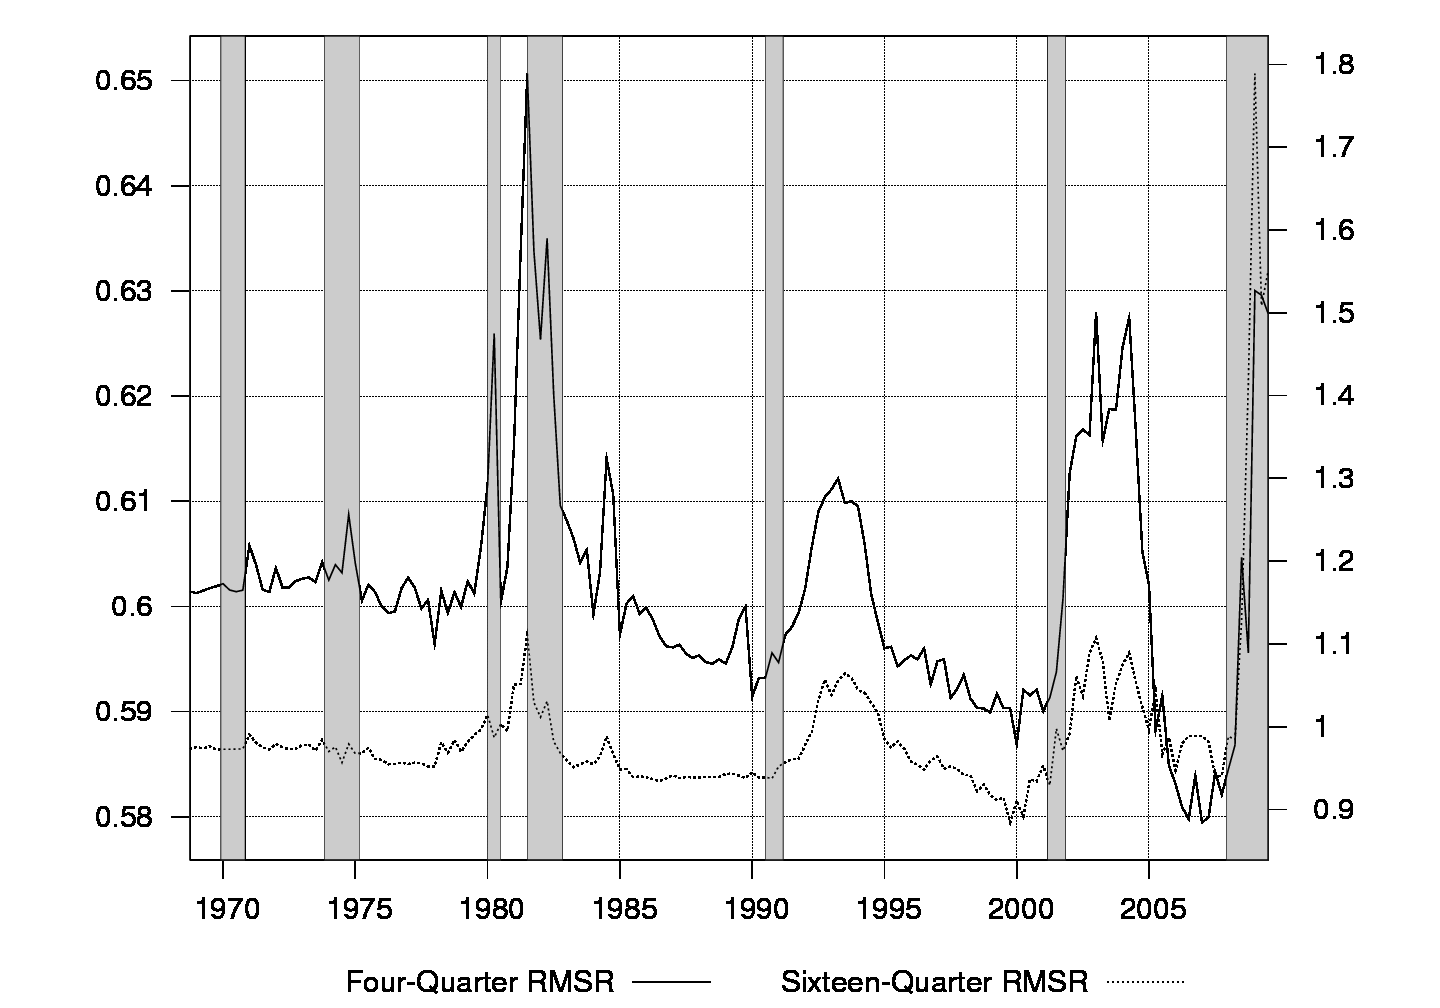
\includegraphics[scale=0.17]{images/RMS16_Output_Gap_Natural_Rate_Shock.png} & 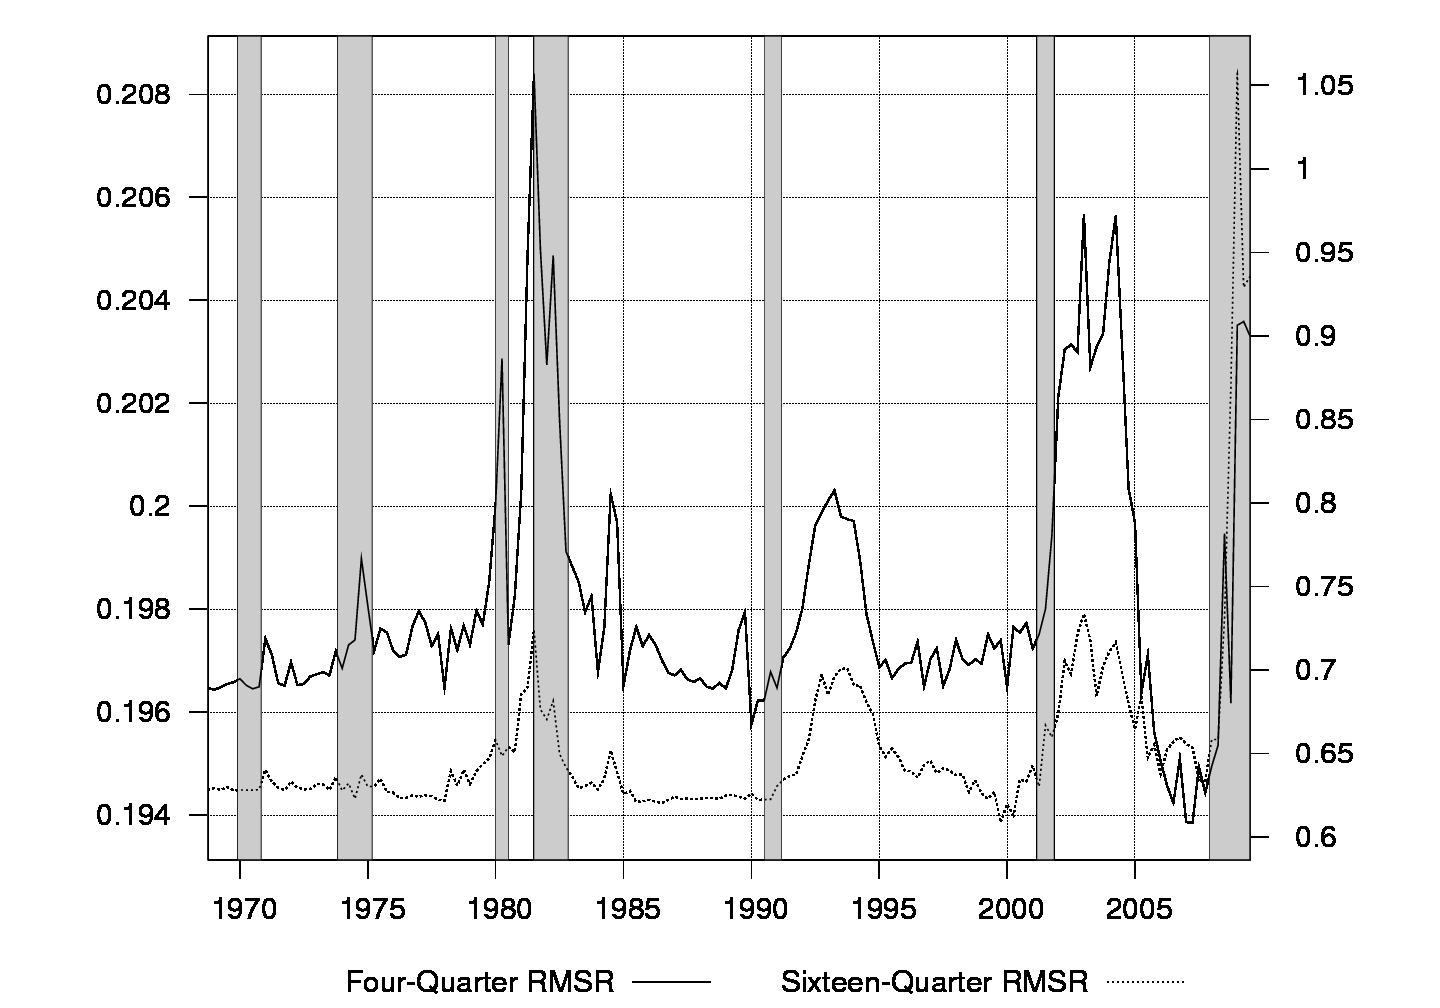
\includegraphics[scale=0.17]{images/RMS16_Inflation_Natural_Rate_Shock.png} \\\\
\textbf{Output Gap Response} & \textbf{Inflation Response} \\
\textbf{to Cost Shock} & \textbf{to Cost Shock}  \\
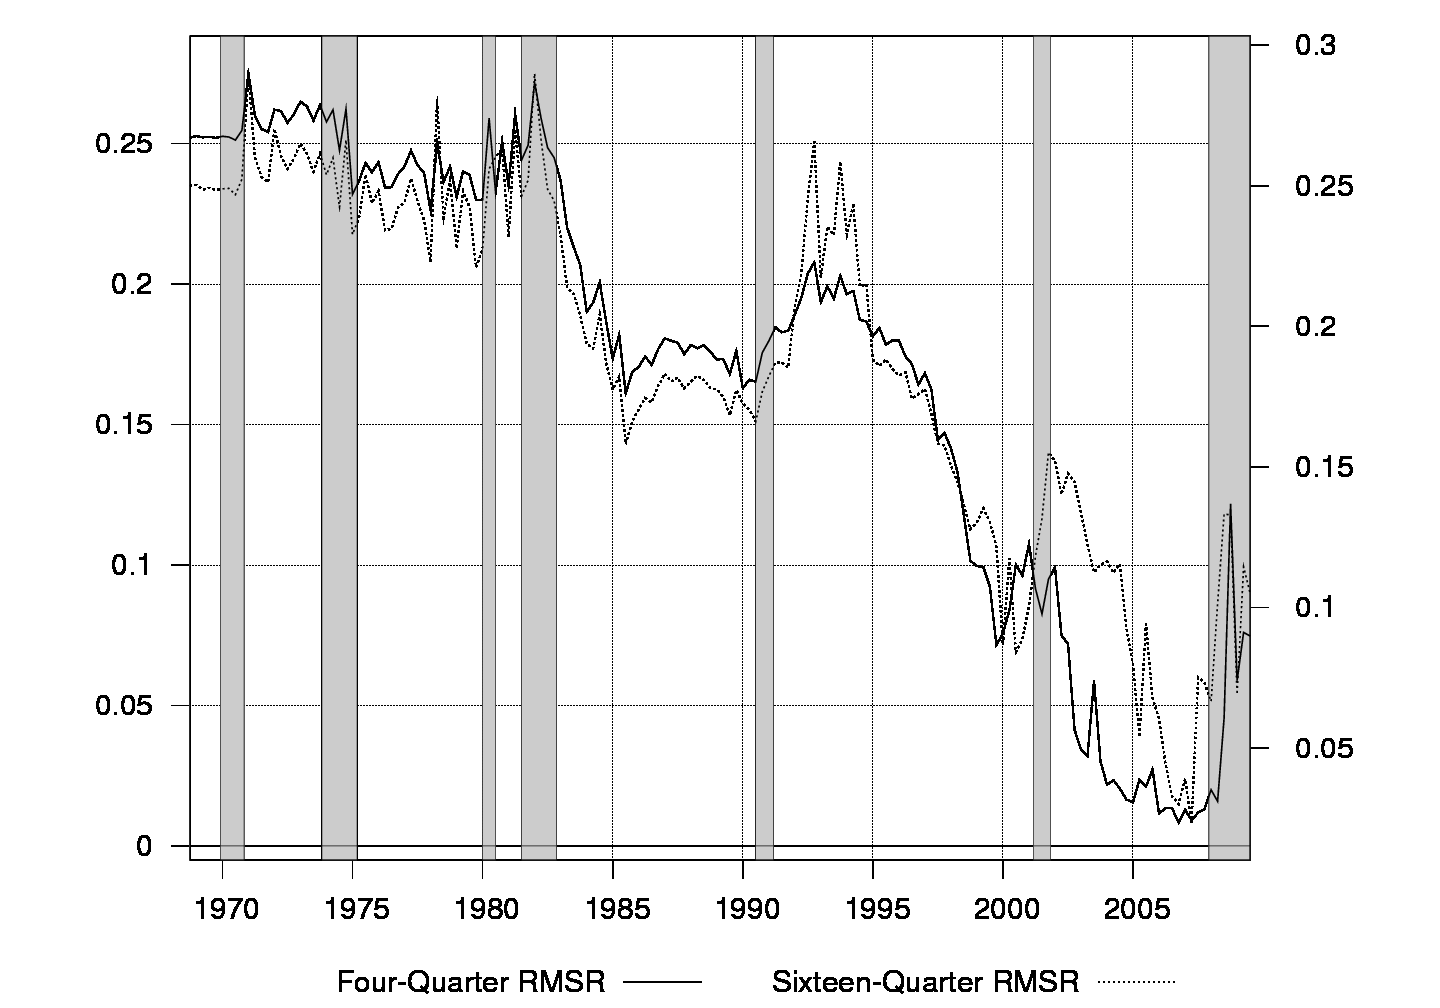
\includegraphics[scale=0.17]{images/RMS16_Output_Gap_Cost_Shock.png} & 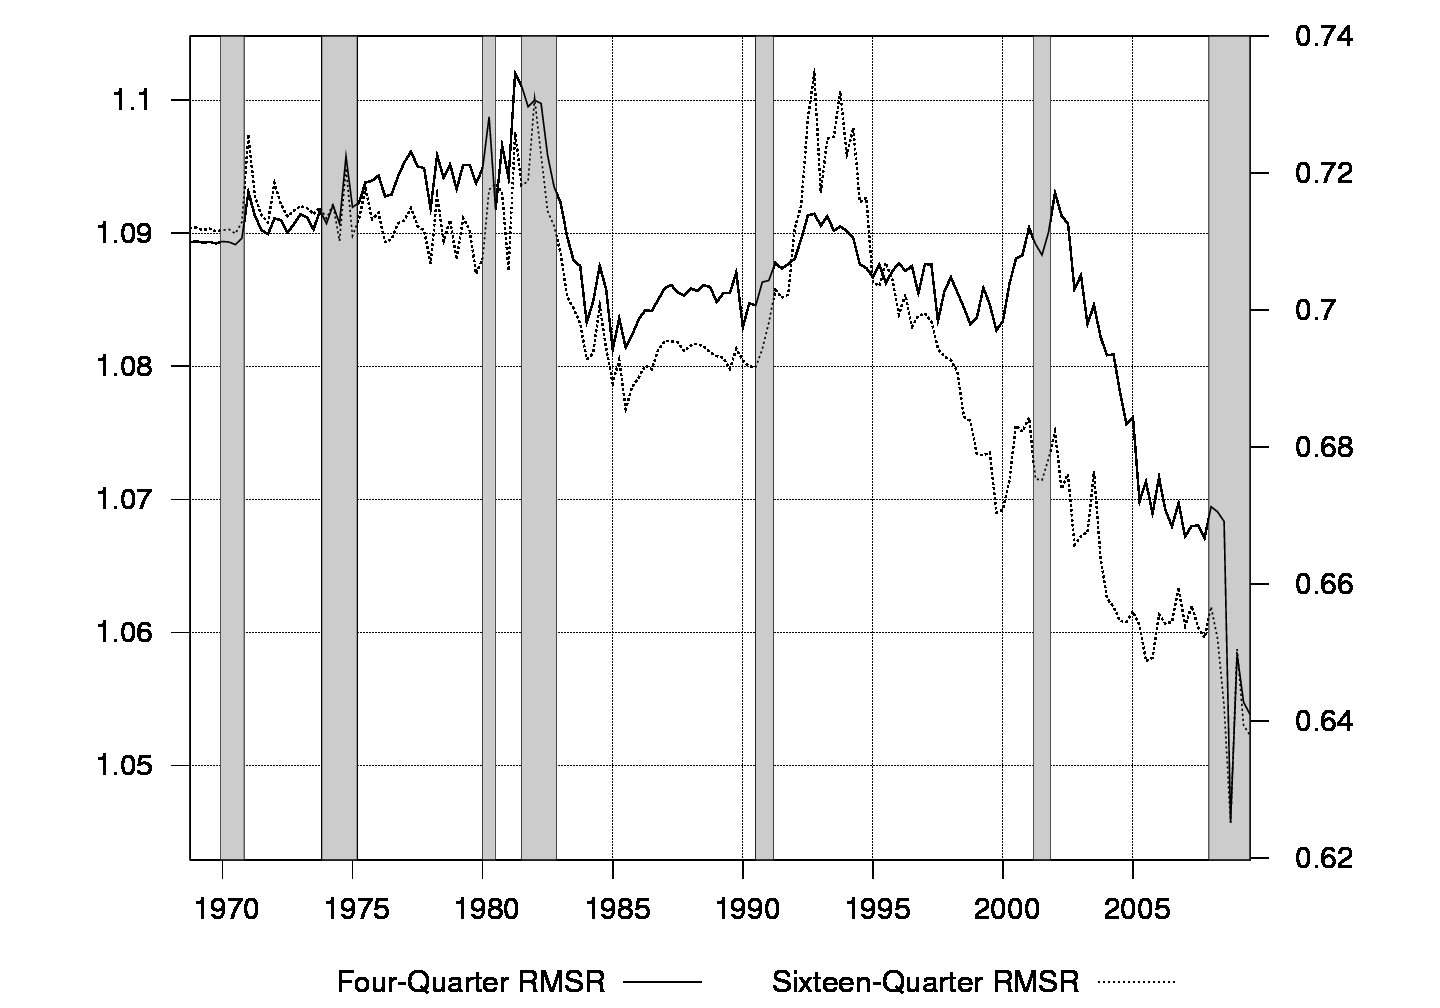
\includegraphics[scale=0.17]{images/RMS16_Inflation_Cost_Shock.png} \\\\
\textbf{Output Gap Response} & \textbf{Inflation Response} \\
\textbf{to Monetary Policy Shock} & \textbf{to Monetary Policy Shock}  \\
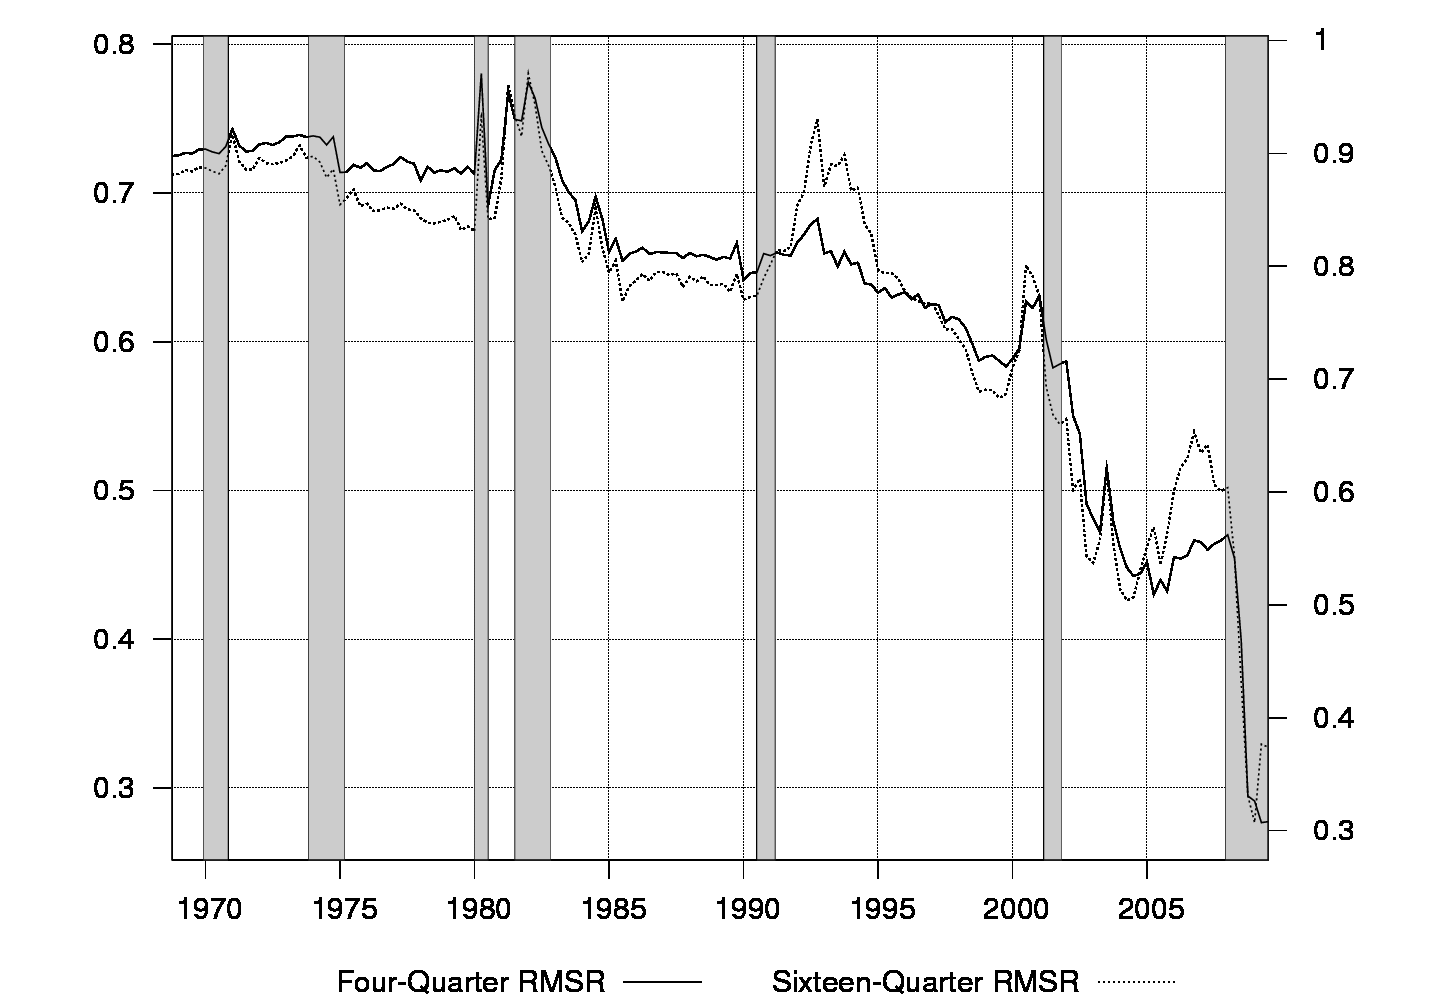
\includegraphics[scale=0.17]{images/RMS16_Output_Gap_Monetary_Policy_Shock.png} & 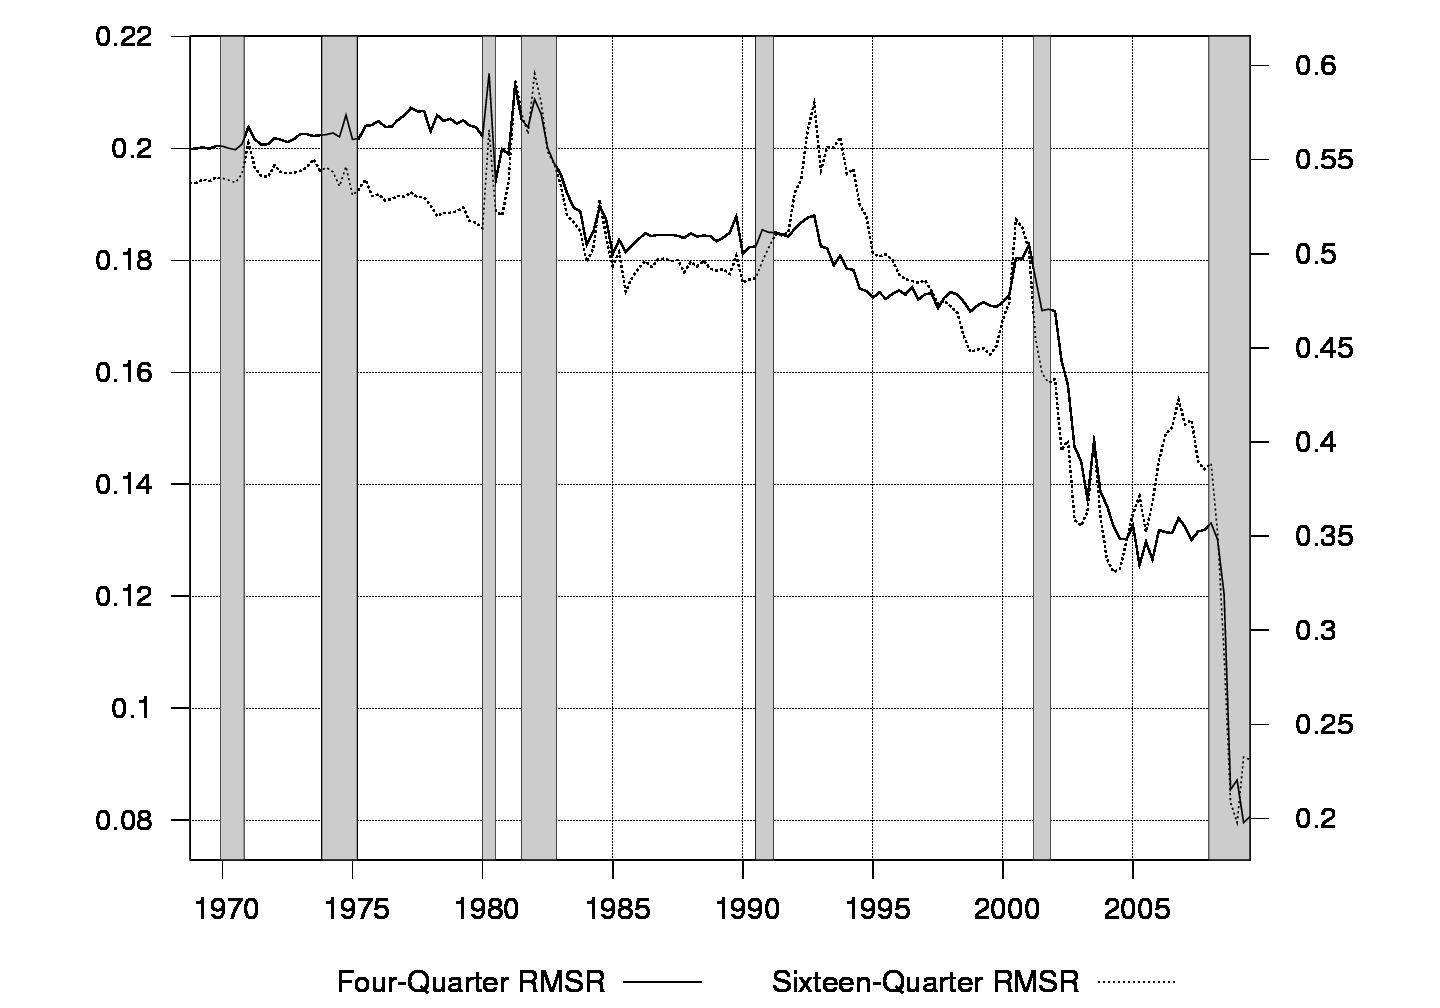
\includegraphics[scale=0.17]{images/RMS16_Inflation_Monetary_Policy_Shock.png} 
\end{tabular}
\end{figure}

\end{document}



